\documentclass[10pt,t]{beamer}
\usetheme{Heverlee}

%\usepackage[orientation=landscape,size=custom,width=16,height=9,scale=0.45,debug]{beamerposter}

\usepackage{svg}
\usepackage{adjustbox}
\usepackage{amsmath,amssymb}
\usepackage{bm}
\usepackage{tikz} % serve per fare i grafici
\usetikzlibrary{shapes,quotes,arrows.meta}
\usepackage{xcolor}
\usepackage{subcaption}
\usepackage{graphicx}
\usepackage{tabularx}
\usepackage{siunitx}
\usepackage{colortbl}

%%% QUICK OPTIONS:
% (A) Math font without serifs, enable line below to make math serif:
    %\usefonttheme[onlymath]{serif}

% (B) Re-define primary colour by adjusting the RGB values
    %\definecolor{pblue}	{RGB}{206,125,66}

% (C) Title page graphic (optional) --- this is not for the background image, see \usebackgroundtemplate to change that ---
    %\titlegraphic{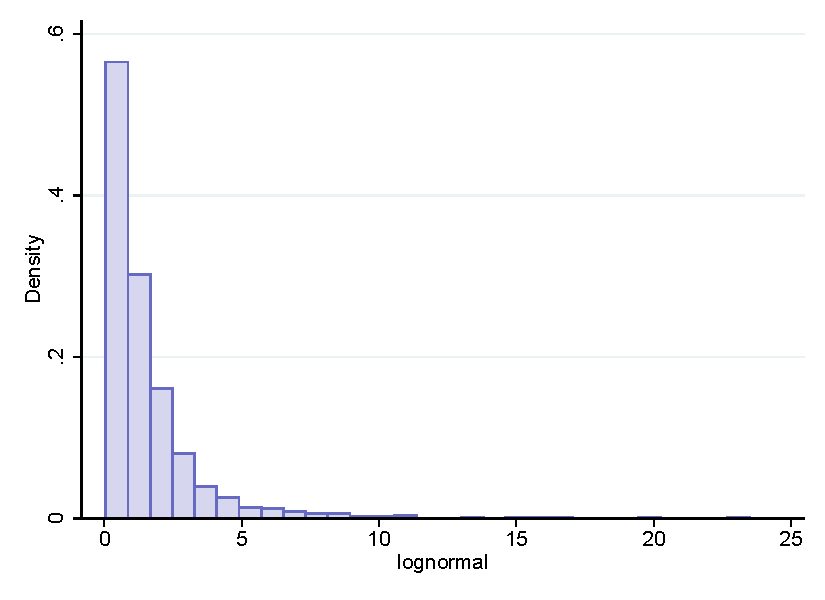
\includegraphics[height=2.7cm]{example_figure.pdf}}

% (D) Add logo to bottom right-corner (optional)
    \logo{
\includegraphics[height=0.82cm]{images/logo-polimi.png}\hspace{8pt}\vspace{-6pt}}      

% (E) Choose one (or none) of these lines to add footline bar on all frames
    %\setbeamertemplate{footline}[infoline]  % author, title, insitute
    %\setbeamertemplate{footline}[navigation] % dots swhowing progress
    %\setbeamertemplate{footline}[navsym] % navigation symbols

% (F) Widescreen 16:9 ratio
    %\usepackage[orientation=landscape,size=custom,width=16,height=9,scale=0.45,debug]{beamerposter} 


\setbeamertemplate{footline}[navigation]
\setbeamertemplate{caption}[numbered]

%%% TITLE PAGE INFO:
\title[Heverlee \LaTeX\ Beamer theme]{Fluid-Structure Interaction}
\subtitle{based on co-simulation with Multibody Dynamics}
\author{Claudio Caccia}
\institute{Politecnico di Milano}
\date{December 2020}

% Text inside {} is used on the title page. Text inside [] is optional, and is used in footline bar (if [] is omitted then text from {} will be used in both ; if [] is specified but left empty then the footline will not show any text)



\makeatletter
\let\beamer@writeslidentry@miniframeson=\beamer@writeslidentry%
\def\beamer@writeslidentry@miniframesoff{%
  \expandafter\beamer@ifempty\expandafter{\beamer@framestartpage}{}% does not happen normally
  {%else
    % removed \addtocontents commands
    \clearpage\beamer@notesactions%
  }
}
\newcommand*{\miniframeson}{\let\beamer@writeslidentry=\beamer@writeslidentry@miniframeson}
\newcommand*{\miniframesoff}{\let\beamer@writeslidentry=\beamer@writeslidentry@miniframesoff}
\makeatother




 %%
 %%  0. TITLE PAGE and TABLE OF CONTENT
 %%
\begin{document}
% Title page

% Change image, or delete this line to remove background image
% TODO get image

%{\usebackgroundtemplate{ \parbox[b][\paperheight][b]{\paperwidth}{\centering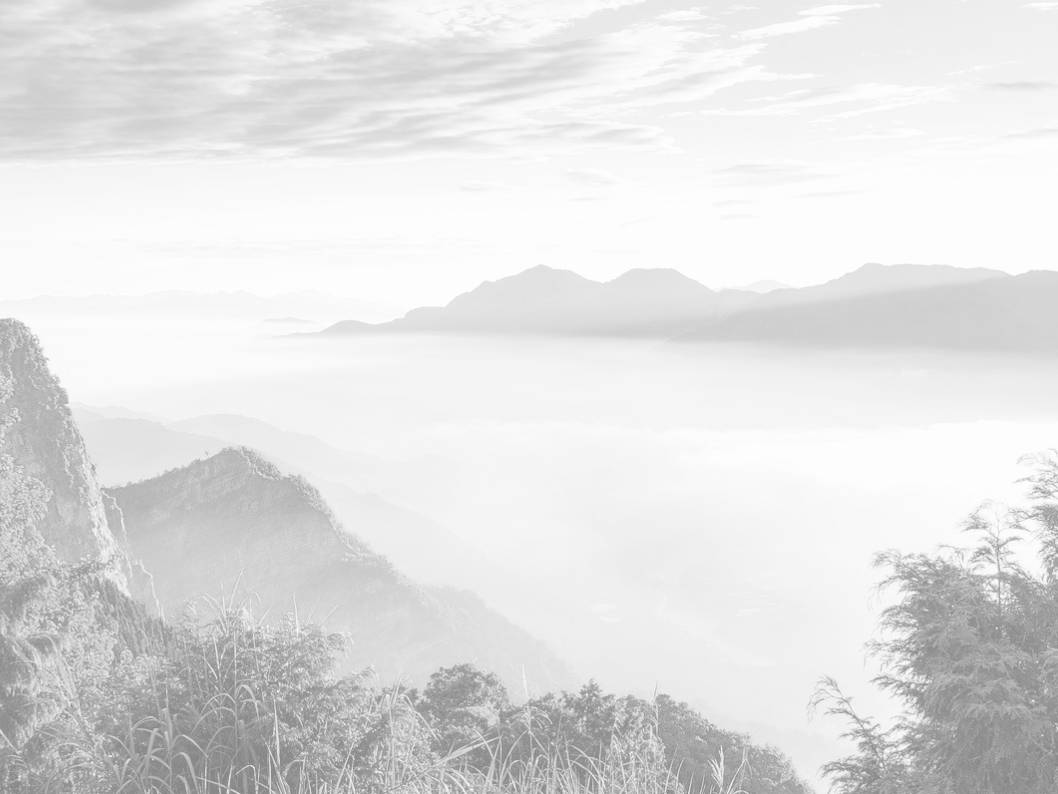
\includegraphics[width=\paperwidth]{Background/bg_alishan.jpg}}} 
 %   abudhabi      cherry      forest      river
 %   alishan       chobe       leuven      sanfancisco
 %   blueprint     columns     library     uyuni
 %   bokeh         flowers     newyork     winter

%\setbeamercolor{background canvas}{bg=lgray}  % make background light gray

%\begin{frame}[plain,noframenumbering]
%    \titlepage
%\end{frame}
%}		

{\usebackgroundtemplate{ \parbox[b][\paperheight][b]{\paperwidth}{\centering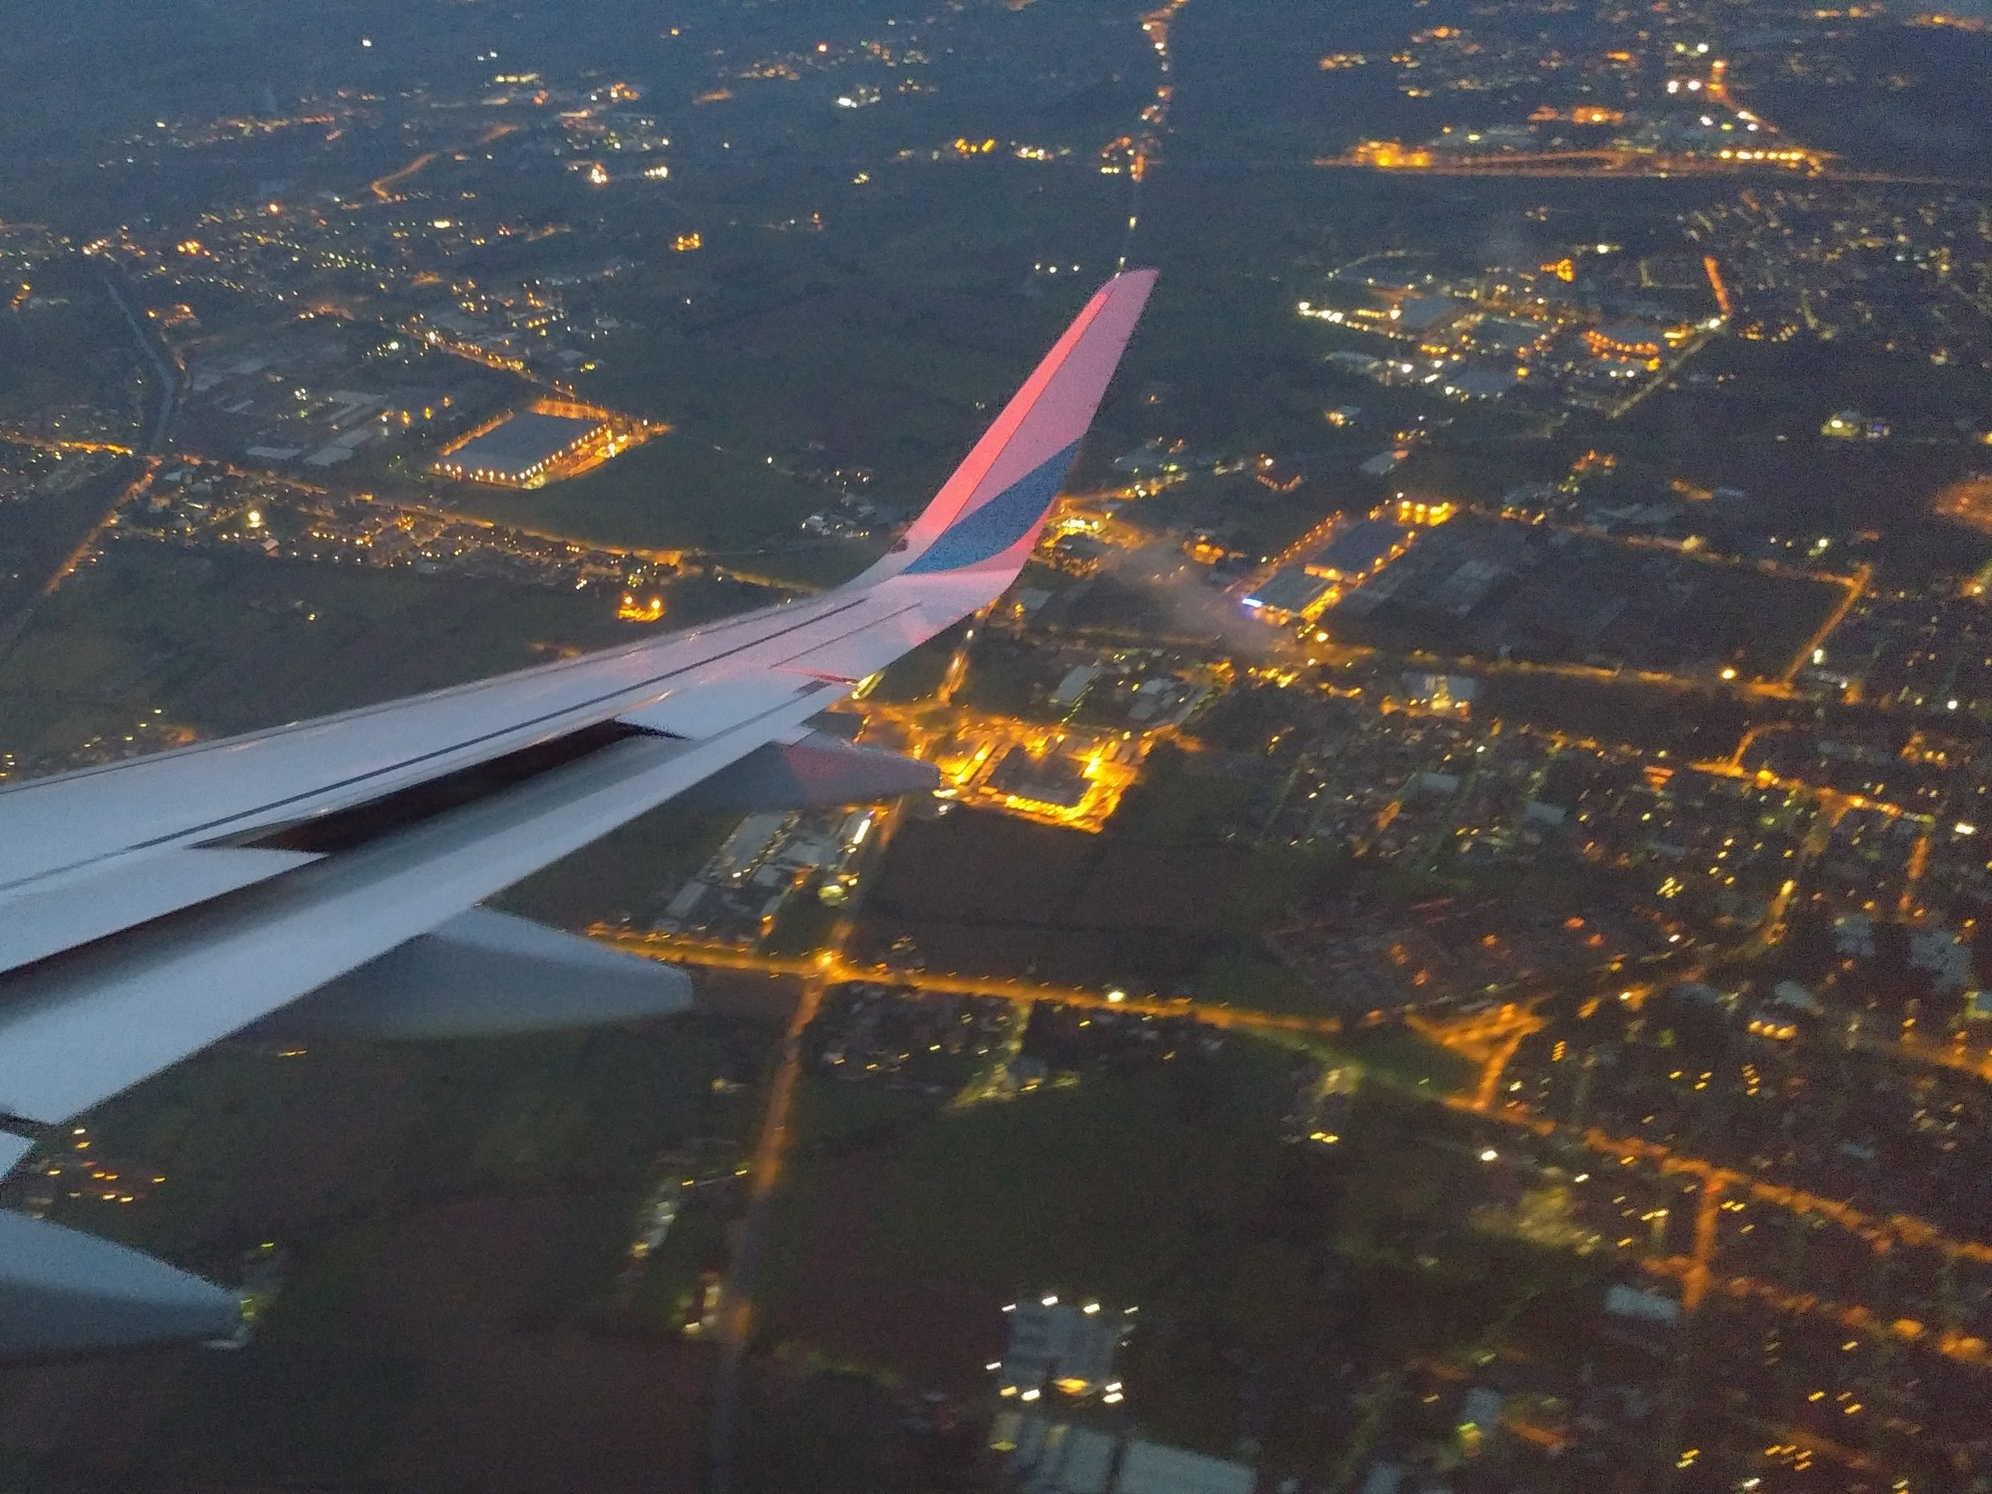
\includegraphics[width=\paperwidth]{Personal_BG/ew07mc.jpg}}} 
\begin{frame}[plain,noframenumbering]
    \titlepage
\end{frame}
}


% Table of contents slide
\begin{frame}{Outline}
	\vskip 2mm
	%Pipolauro?
	\vskip 2mm
	\hfill	{\large \parbox{.95\textwidth}{\tableofcontents[hideothersubsections]}}
\end{frame}


% SECTION 1
\section[FSI techniques]{FSI solution techniques}




\begin{frame}{FSI}
What is FSI?

    \begin{itemize}
        \item fluid forces change the shape of the structure
        
        \item structure deformation changes the fluid domain and the flow
    \end{itemize}
    

    \begin{columns}
        \column{0.5\textwidth}
        \begin{figure}
            \centering
            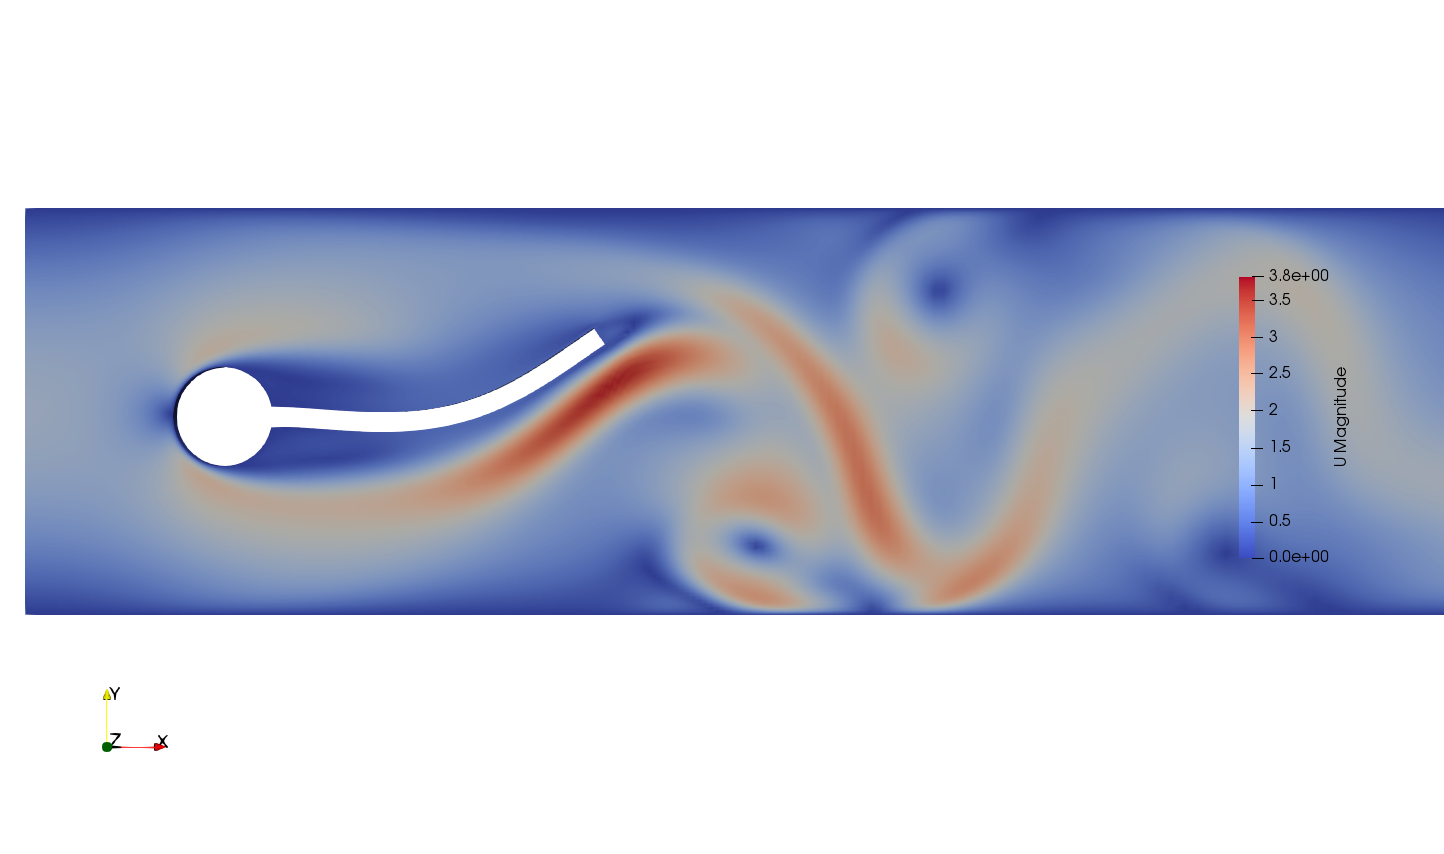
\includegraphics[width=0.95\textwidth,trim=0 100 0 100,clip]{images/flap1.png}
            \caption{cylinder flap}
        \end{figure}
        \column{0.5\textwidth}
        \begin{figure}
            \centering
            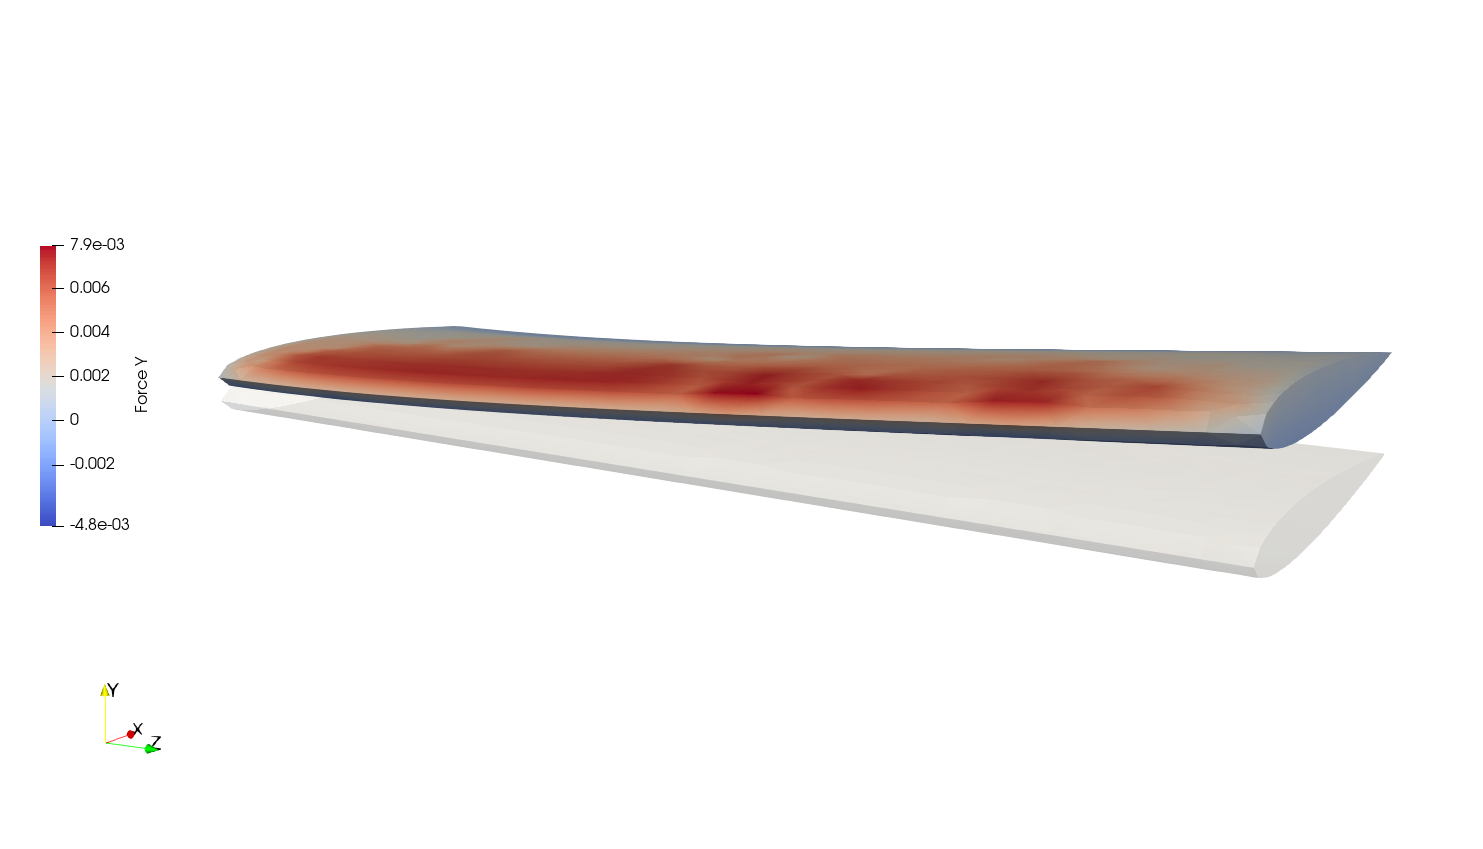
\includegraphics[width=0.95\textwidth,trim=0 100 0 100,clip]{images/naca.png}
            \caption{wing deformation}
        \end{figure}
    \end{columns}
    
    \pause
    
    
    \vskip 5mm
    
   \textcolor{red}{Fluid and solid interact and need to be simulated together}
    
    
\end{frame}






\begin{frame}{solution techniques}

%\begin{columns}
%    \column{0.6\textwidth}

\vspace{5mm}
\begin{block}{Monolithic Approach}
\begin{figure}[htbp!]
	\centering
	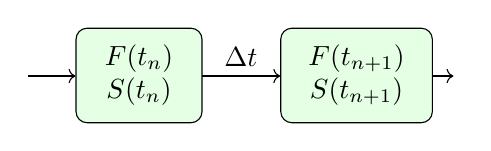
\begin{tikzpicture}[scale=1]
        \tikzstyle{status}=[draw,rectangle,rounded corners,fill=green!10,text centered,inner sep=4pt, anchor=south west, minimum width=1.6cm,minimum height=1.2cm]
	    
	    \draw[->] (0,0.6)-- (0.6,0.6) node[] {};
	    
	    \draw[->] (2.2,0.6)-- (3.2,0.6) node[midway,above] {$\Delta t$}; % node[midway,below] {step};
        
	    \draw[->] (4.8,0.6)-- (5.4,0.6) node[] {};

	    \node[status] (t1) at (0.6,0)  {
		    \begin{tabular}{c}
			    $F(t_n)$ \\
			    $S(t_n)$
	        \end{tabular}};
        
        \node[status] at (3.2,0) {
	        \begin{tabular}{c}
		        $F(t_{n+1})$ \\
		        $S(t_{n+1})$
            \end{tabular}};
	
	\end{tikzpicture}
\end{figure}
\end{block}

\pause
\vspace{5mm}
%\column{0.4\textwidth}
    \begin{itemize}
        \itemsep 5pt
        \item \textcolor{teal}{\textbf{shared interface}}
        \item specialized \textit{ad hoc} solver
        \item difficult to develop and maintain
    \end{itemize}

%\end{columns}

\end{frame}

\begin{frame}{Solution techniques}

\begin{exampleblock}{Partitioned Approach}

\begin{figure}[htbp!]
	\centering
	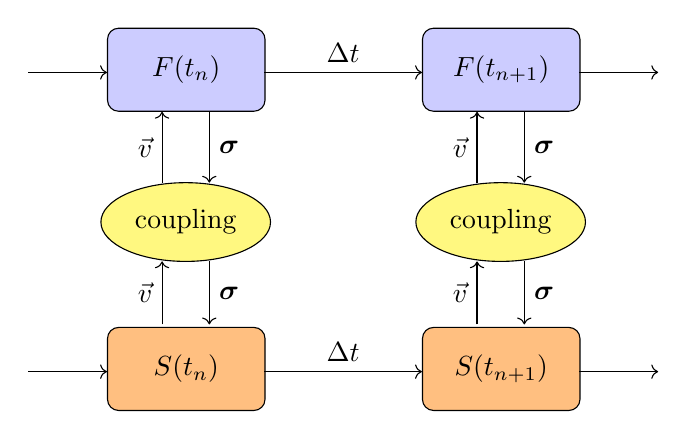
\begin{tikzpicture}[scale=1]

	\tikzstyle{solver}=[draw,rectangle,rounded corners,text centered,inner sep=10pt, anchor=south west, minimum width=2cm,minimum height=1cm]
	\tikzstyle{coupling}=[draw, ellipse, fill=yellow!75, minimum width=2cm, minimum height=1cm, align=center]

	\node[solver,fill=blue!20] at (1,3.8) {$F(t_n)$};
	\node[solver,fill=blue!20] at (5,3.8) {$F(t_{n+1})$};
	
	\node[solver,fill=orange!50] at (1,0) {$S(t_n)$};
	\node[solver,fill=orange!50] at (5,0) {$S(t_{n+1})$};
	
	\draw[->] (0,0.5)-- (1,0.5) node[] {};
	\draw[->] (3,0.5)-- (5,0.5) node[midway,above] {$\Delta t$}; % node[midway,below] {step};
	\draw[->] (7,0.5)-- (8,0.5) node[] {};


	\draw[->] (0,4.3)-- (1,4.3) node[] {};
	\draw[->] (3,4.3)-- (5,4.3) node[midway,above] {$\Delta t$}; % node[midway,below] {step};
	\draw[->] (7,4.3)-- (8,4.3) node[] {};
	
	\node[draw,fill=yellow!50,ellipse,minimum width=2cm, minimum height=1cm] at (2,2.4) {coupling};
	\node[draw,fill=yellow!50,ellipse,minimum width=2cm, minimum height=1cm] at (6,2.4) {coupling};

	\draw[->] (1.7,1.1)-- (1.7,1.9) node[midway,left] {$\vec{v}$};
	\draw[->] (2.3,1.9)-- (2.3,1.1) node[midway,right] {$\bm{\sigma}$};

	\draw[->] (1.7,2.9)-- (1.7,3.8) node[midway,left] {$\vec{v}$};
	\draw[->] (2.3,3.8)-- (2.3,2.9) node[midway,right] {$\bm{\sigma}$};

	\draw[->] (5.7,1.1)-- (5.7,1.9) node[midway,left] {$\vec{v}$};
	\draw[->] (6.3,1.9)-- (6.3,1.1) node[midway,right] {$\bm{\sigma}$};

	\draw[->] (5.7,2.9)-- (5.7,3.8) node[midway,left] {$\vec{v}$};
	\draw[->] (6.3,3.8)-- (6.3,2.9) node[midway,right] {$\bm{\sigma}$};
		
	\end{tikzpicture}
	%\caption{partitioned approach: $S_f$, $S_s$ denote the fluid and the structure solutions, while $\bm{\sigma}$ and $\vec{v}$ represent coupling data}
	%\label{fig:partitioned}
\end{figure}
\end{exampleblock}

\end{frame}


\begin{frame}{Partitioned Approach}
    \begin{itemize}
        \item  3 Different software modules
            \begin{enumerate}
                \itemsep 5pt
                \item \textbf{CFD} solver
                \item \textbf{CSM} solver
                \item coupling software for \textcolor{red}{data exchange}
            \end{enumerate}
        \vspace{5mm}
        \pause
        \item Software modularity is preserved
        \item Reuse of existing \textcolor{red}{validated} solvers
        
        \vspace{5mm}
        \pause
        
        \item The interface is no longer shared
        
        \begin{enumerate}
            \itemsep 5pt
            \item coupling must be enforced (\textcolor{teal}{equilibrium} and \textcolor{pblue}{compatibility})
            \item the solution is \textcolor{red}{exact} up to some convergence criteria
        \end{enumerate}
    \end{itemize}
\end{frame}


\begin{frame}{Weak vs. strong coupling}

\begin{block}{Weak coupling}
Solvers:
\begin{itemize}
    \item \textcolor{dblue}{compute}
    \item \textcolor{fgreen}{exchange data}
    \item \textcolor{dorange}{advance} 
\end{itemize}
No convergence criteria are applied. It might be unstable.
\end{block}

\pause

\vspace{5mm}
\begin{exampleblock}{Strong coupling}
Solvers iterate \textcolor{dblue}{computation} and \textcolor{fgreen}{data exchange} until some convergence criteria are met. Then \textcolor{dorange}{advance} to next time step.
\end{exampleblock}
\label{coupling}
\hyperlink{couplingdetails}{\beamergotobutton{Coupling math details}}

\end{frame}

\begin{frame}{Added Mass Instability}
\label{addedmass}
\begin{alertblock}{convergence issues}
A critical simulation parameter

\begin{center}
    \textcolor{red}{\textbf{mass ratio}}: $M = \frac{\rho_F}{\rho_S}$ 
\end{center}

    


\vspace{0.1cm}
\textbf{critical} when $\approx 1$
\vspace{0.1cm}


\end{alertblock}

\vspace{0.8cm}

    \begin{itemize}
        \item \textbf{Weak coupling} may \textcolor{red}{diverge}
        \item \textbf{Strong coupling} requires \textcolor{dorange}{many iterations} to converge or may \textcolor{red}{diverge}
    \end{itemize}

\vspace{0.8cm}


\hyperlink{dimensionless}{\beamergotobutton{Other dimensionless numbers}}

\end{frame}





\section{MBDyn and preCICE}

\begin{frame}{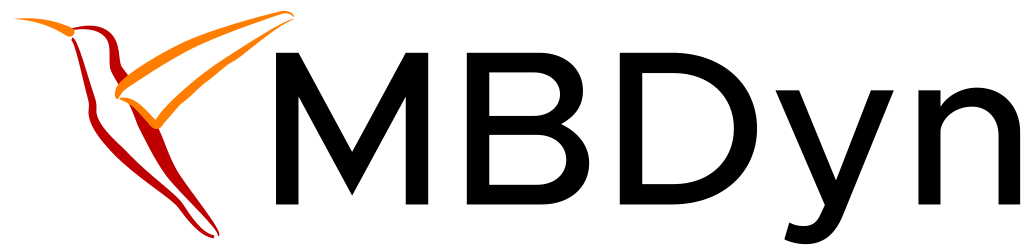
\includegraphics[width=.18\textwidth]{images/mbdyn.png} }

\textbf{\textcolor{dorange}{M}ulti\textcolor{dorange}{B}ody \textcolor{red}{DYN}amics analysis} software (\url{www.mbdyn.org}).\\


\vspace{5mm}

Main features:

    \begin{itemize}
        \item simulation of linear and non-linear \textbf{\textcolor{dorange}{dynamics}}
        \item definition of rigid and flexible elements:\\ \textbf{\textcolor{dblue}{beams}}, shells, component mode synthesis elements...
        \item subject to \textbf{\textcolor{pblue}{kinematic constraints}} and \textbf{\textcolor{indigo}{external forces}}
        \item possibly governed by \textbf{\textcolor{fgreen}{control subsystems}}
    \end{itemize}

\pause
\vspace{5mm}

Open to perform multi-physics simulations:
\begin{itemize}
    \item \textcolor{teal}{\textbf{map}} between \textit{nodes} and external points:
    \begin{itemize}
    \footnotesize
        \item \textcolor{fgreen}{\textbf{pass}} externally computed forces to MBDyn
        \item \textcolor{indigo}{\textbf{retrieve}} point displacements
    \end{itemize}
    \normalsize
    \item \textcolor{teal}{\textbf{steer}} the simulation
\end{itemize}

\end{frame}


\begin{frame}{External Structural Mapping}

\textcolor{red}{Decoupling geometry and structural properties:} 

\begin{figure}
  \begin{subfigure}[t]{.486\textwidth}
    \centering
    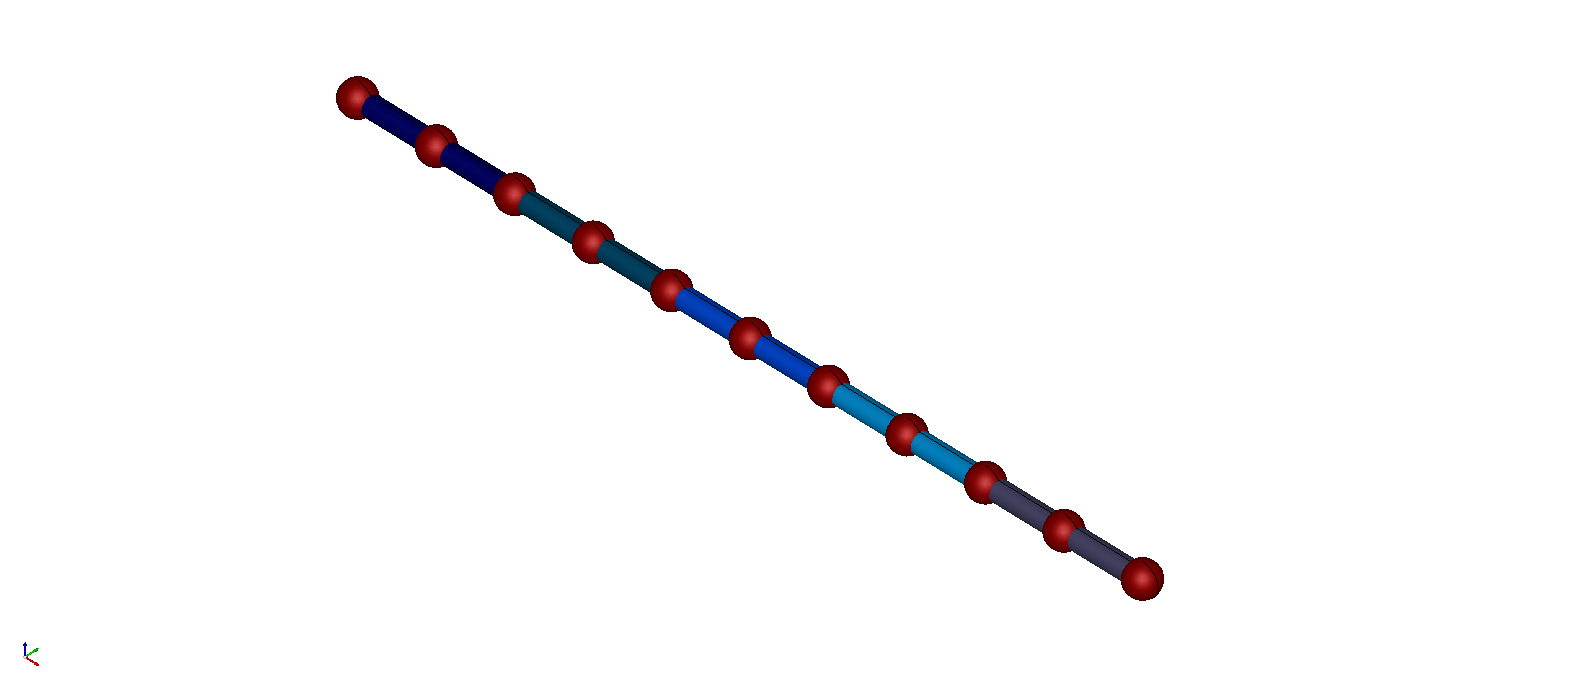
\includegraphics[width=\linewidth]{images/beams_1a.png}
    \caption{Model: \textbf{nodes} and \textbf{beams}}
  \end{subfigure}
  \hfill
  \begin{subfigure}[t]{.486\textwidth}
    \centering
    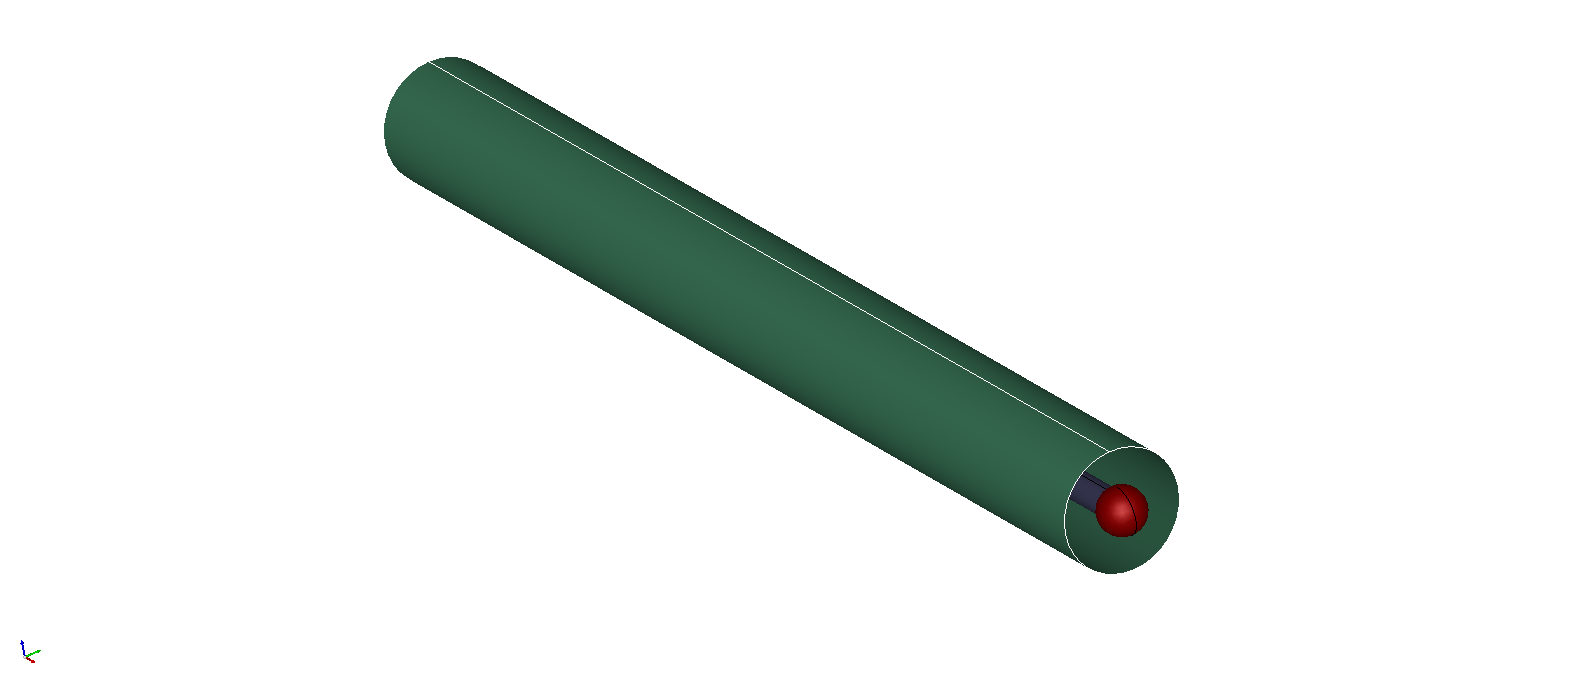
\includegraphics[width=\linewidth]{images/interf_1a.png}
    \caption{interface geometry: \textbf{shape}}
  \end{subfigure}

  \bigskip

  \begin{subfigure}[t]{.486\textwidth}
    \centering
    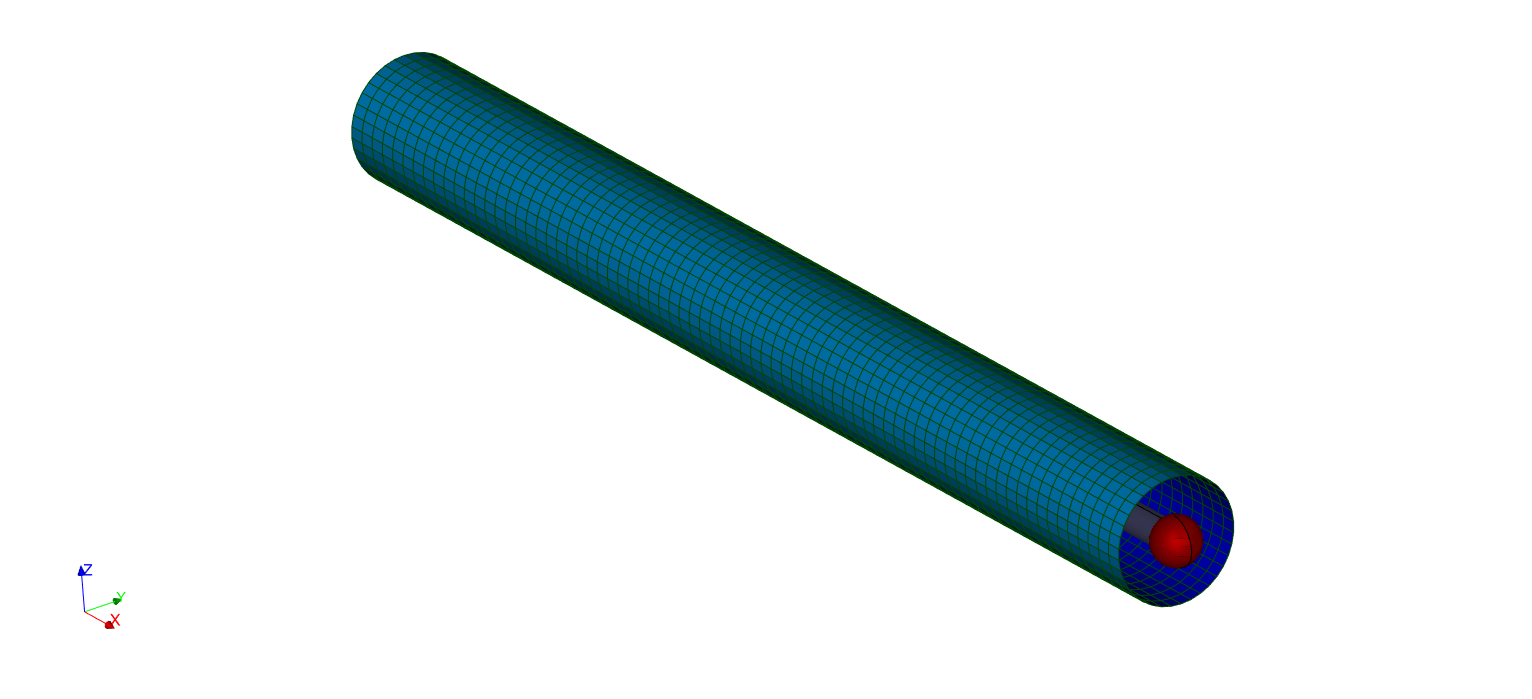
\includegraphics[width=\linewidth]{images/mesh_1b.png}
    \caption{interface mesh: \textbf{MLS mapping}}
  \end{subfigure}
  \hfill
  \begin{subfigure}[t]{.486\textwidth}
    \centering
    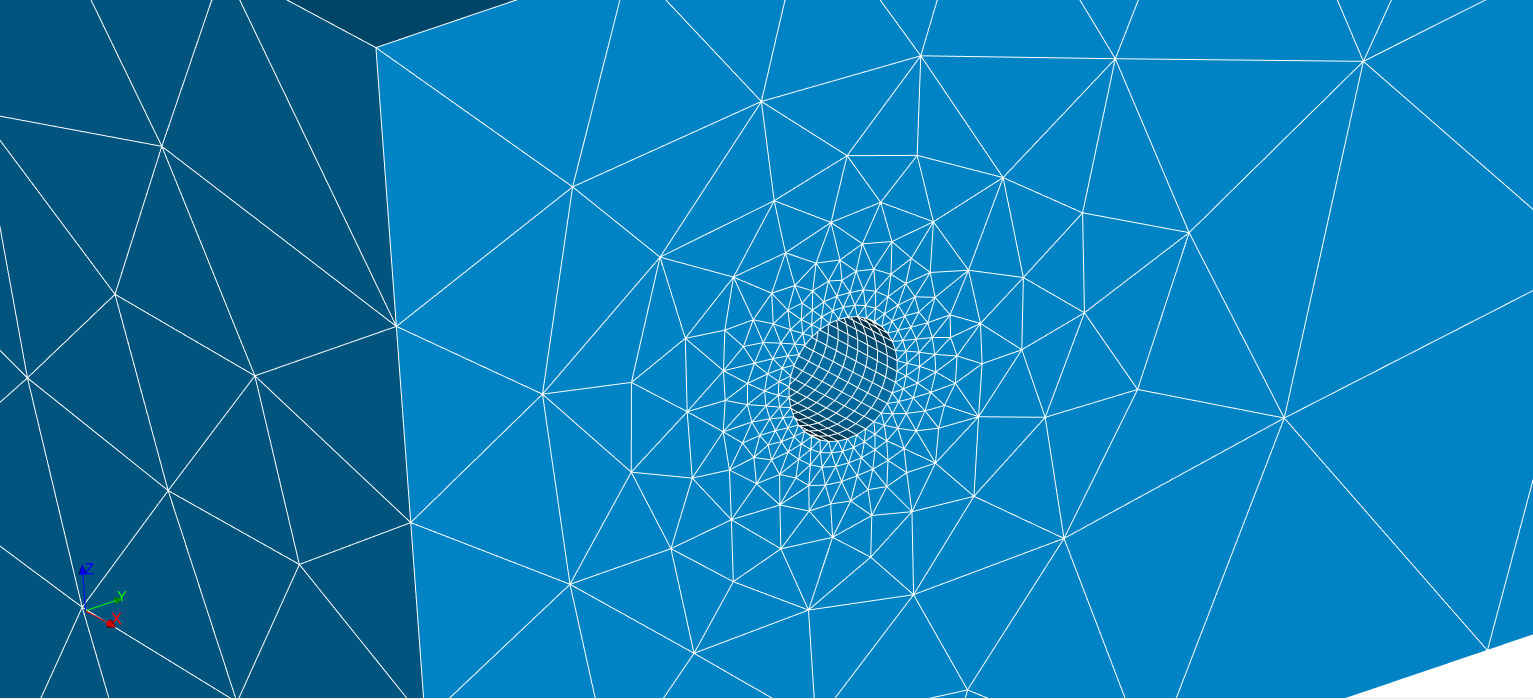
\includegraphics[width=\linewidth]{images/whole_1aa.png}
    \caption{\textbf{coupling} to CFD solver}
  \end{subfigure}
\end{figure}


\end{frame}



\begin{frame}{
\includegraphics[width=.22\textwidth]{images/precice.png}}

\textbf{\textcolor{dorange}{pre}cise \textcolor{pblue}{C}ode \textcolor{pblue}{I}nteraction \textcolor{pblue}{C}oupling \textcolor{pblue}{E}nvironment} (\url{www.precice.org})

%\pause
\vspace{5mm}

Main features:

    \begin{itemize}
        \item connection of single-physics solvers
        \item partitioned multi-physics simulation: FSI, CHT, SSI
        \item black-box: information only on interface nodes 
    \end{itemize}

\pause
\vspace{5mm}

Actions performed: 

\begin{itemize}
	\item coupling strategy
	\item acceleration and convergence criteria
	\item communication between the participants
	\item mapping of data between meshes 
\end{itemize}

\end{frame}



\begin{frame}{FSI Simulations using MBDyn}

\begin{figure}
    \centering
    \begin{tikzpicture}
        \node[inner sep=0pt] (mbdyn) at (0,0)
            {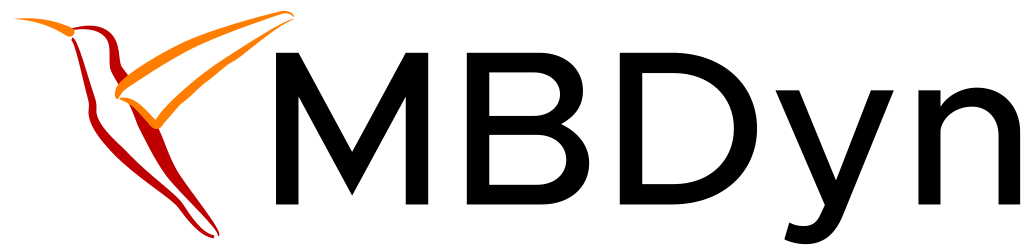
\includegraphics[width=.25\textwidth]{images/mbdyn.png}};
        \node[inner sep=0pt] (precice) at (0,-2.5)
            {
\includegraphics[width=.25\textwidth]{images/precice.png}};
        \node[inner sep=0pt] (of) at (-4,-5) 
            {
\includegraphics[width=.2\textwidth]{images/of.jpeg}};
        \node[inner sep=0pt] (su2) at (-1.25,-5) 
            {
\includegraphics[width=.12\textwidth]{images/logoSU2.png}};
        \node[inner sep=0pt] (cfd) at (0.5,-5) 
            {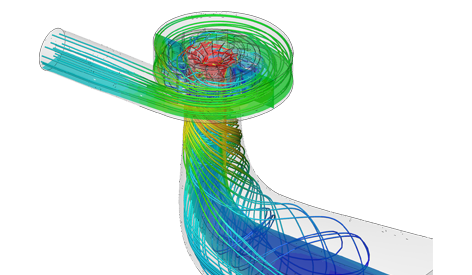
\includegraphics[width=.14\textwidth]{images/simulation-CFD.png}};
        \node[inner sep=0pt] (aster) at (4,-5) 
            {
\includegraphics[width=.125\textwidth]{images/Logo_aster.png}};
        \draw[<->,thick] (mbdyn.south) -- (precice.north)
            node[midway,fill=white,text=orange] {\large{\textbf{adapter}}};
         \draw[->,thick] (precice.south) -- (of.north east)
            node[midway] {};
         \draw[->,thick] (precice.south) -- (su2.north)
            node[midway,fill=white, text=cyan] {\large{\textbf{FSI}}};
         \draw[->,thick] (precice.south) -- (cfd.north)
            node[midway] {};
         \draw[->,thick] (precice.south) -- (aster.north west)
            node[midway,fill=white, text=teal] {\large{\textbf{SSI}}};
            
\end{tikzpicture}
\end{figure}

\end{frame}






\section{Adapter}

\begin{frame}{MBDyn adapter}
    \begin{figure}
        \centering
        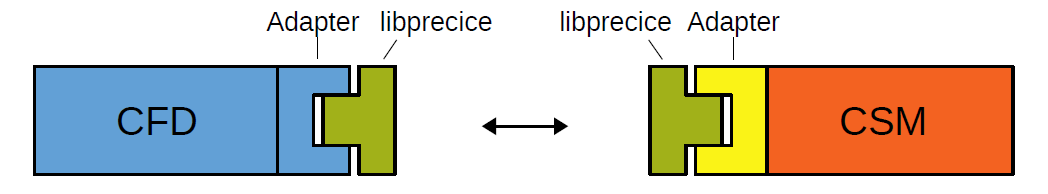
\includegraphics[width=0.8\textwidth]{images/adapter_scheme.png}
    \end{figure}
    
    \vspace{3mm}
    
    \begin{itemize}
     \itemsep 8pt
        \item \textcolor{teal}{\textbf{independent}} from MBDyn code
        \item \textcolor{dblue}{\textbf{APIs}} from preCICE and MBDyn:
        \begin{enumerate}
            \itemsep 5pt
            \item \texttt{libprecice.so}   \hspace{0.6cm} (from MBDyn)
            \item \texttt{libmbc.so}       \hspace{1.27cm}    (from preCICE)
        \end{enumerate}
        
        \item composed of 2 C++ \textcolor{indigo}{\textbf{classes}}:
        \begin{enumerate}
            \itemsep 5pt
            \item perform co-simulation
            \item access and steer the MBDyn simulation, save data
        \end{enumerate}
        
    \end{itemize}
\end{frame}

\begin{frame}{Adapter Input}
  \vspace{1.5cm}
  \begin{description}[Simulation]
  \itemsep 10pt
  \item[preCICE] \textcolor{dorange}{config file, participant name, ...}
  \item[MBDyn]      \textcolor{red}{simulation file} \\
                    \textcolor{red}{socket}: send forces and retrieve displacements \\
  \item[Simulation] \textcolor{teal}{mesh location}: used for coupling and mapping\\
                    \textcolor{teal}{data to pass}: displacements or deltas\\
                    \textcolor{teal}{starting ramp configuration}: type, period, ...
%  \item[Output]     \textcolor{indigo}{vtk file}: location, name, time interval, ...\\
%                    \textcolor{indigo}{resultants}: name, origin for moments, ...
  \end{description}

%    \begin{figure}
%        \centering
%        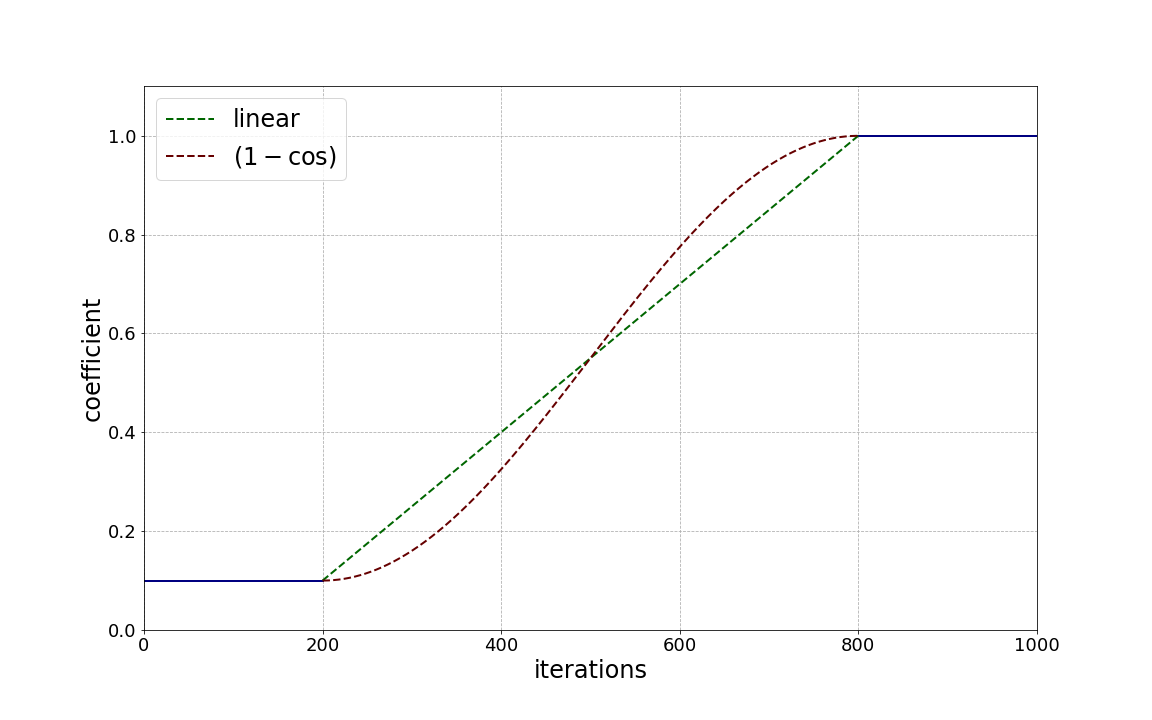
\includegraphics[width=0.5\textwidth, trim=0 45 0 50,clip]{images/coeff_pres.png}
%        \caption{scaling factor at start}
%    \end{figure}

\end{frame}

\begin{frame}{Adapter Output}

\begin{description}[saved data]
    \item[*.vtu files] at each mapped interface point: \\
                    \textcolor{dorange}{Displacements}, \textcolor{red}{Deltas}\\ 
                    \textcolor{dblue}{Velocities}\\
                    \textcolor{teal}{Forces}
    \item[csv file] with resultants and moments at each $\Delta t$
    \item[MDByn] simulation output parsed through \texttt{python} script
\end{description}



\begin{figure}
 \begin{subfigure}[t]{.486\textwidth}
    \centering
    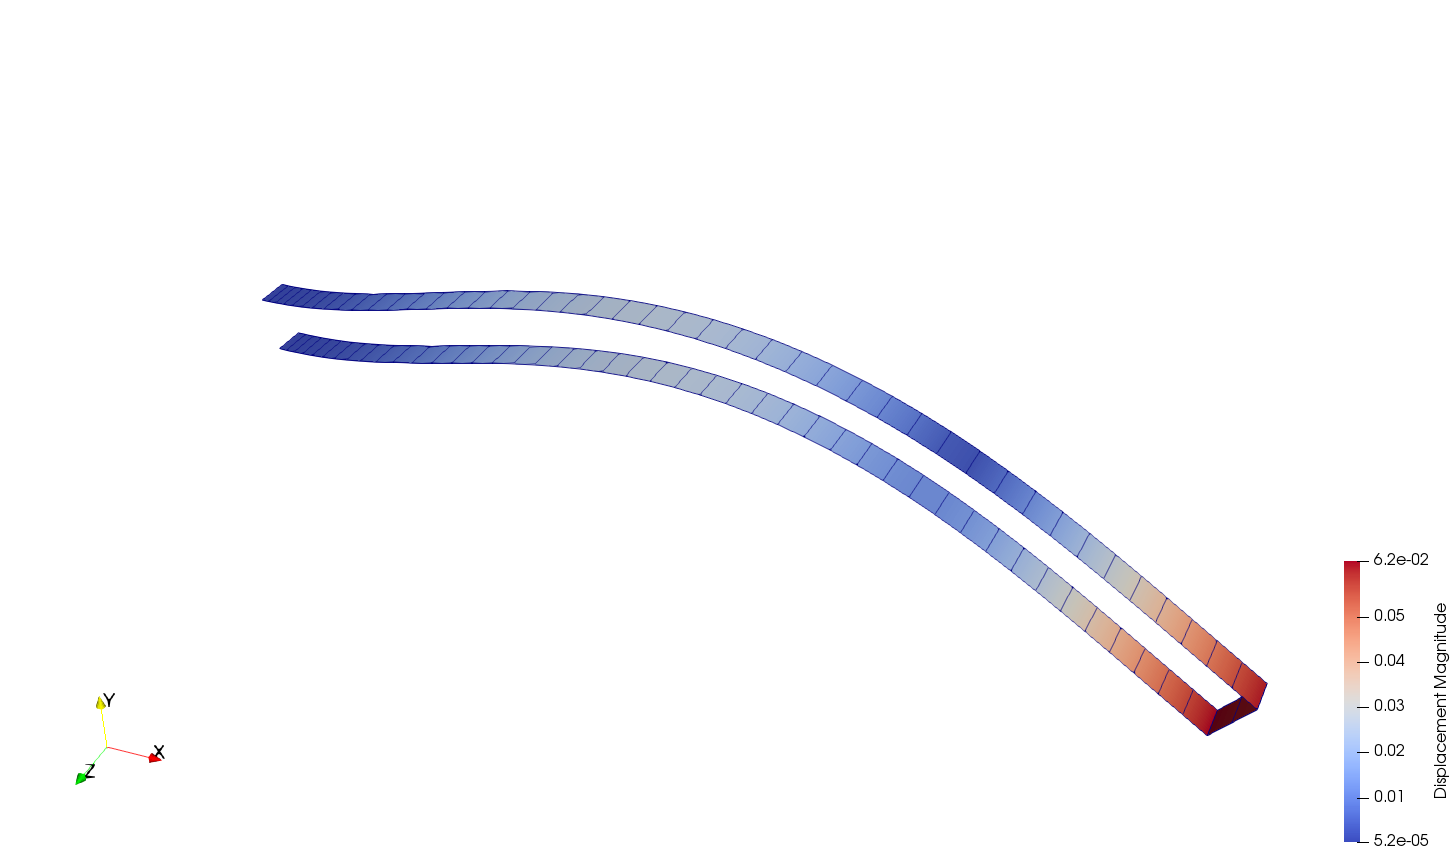
\includegraphics[width=\linewidth, trim=20 0 0 200,clip]{images/fsi2_disp.png}
    \caption{2D FSI example}
  \end{subfigure}
  \hfill
  \begin{subfigure}[t]{.486\textwidth}
    \centering
    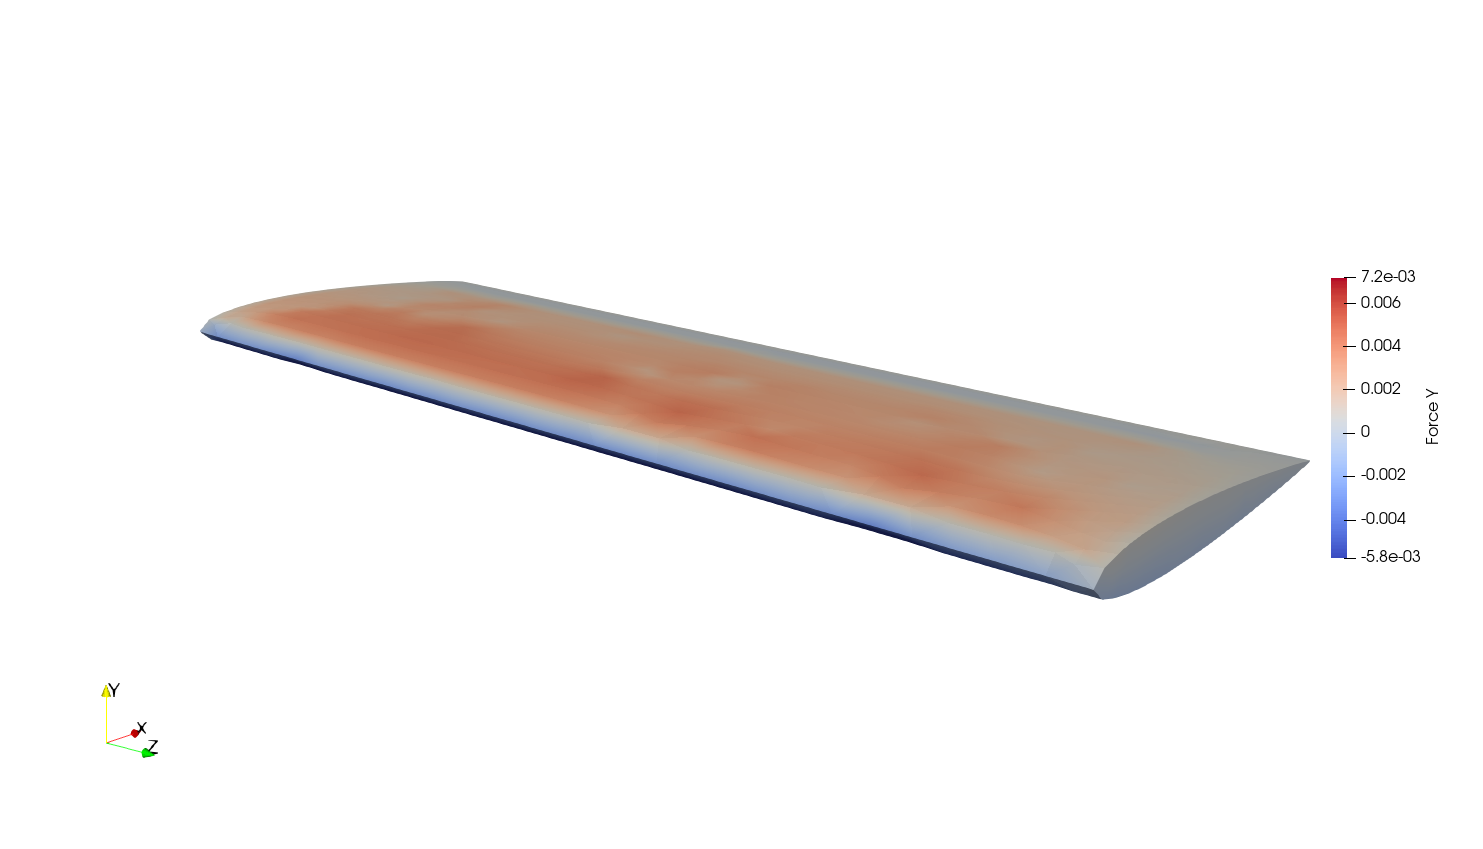
\includegraphics[width=\linewidth]{images/naca_force.png}
    \caption{3D FSI example}
  \end{subfigure}
\end{figure}


\end{frame}



\section{Test Cases}

\begin{frame}{Square Bluff Body (Wall 1998): domain}

\begin{columns}
    \column{0.6\textwidth}
    \begin{figure}[t]
    \vspace*{-1cm}
	\centering
	  \begin{subfigure}[t]{\textwidth}
    \centering
    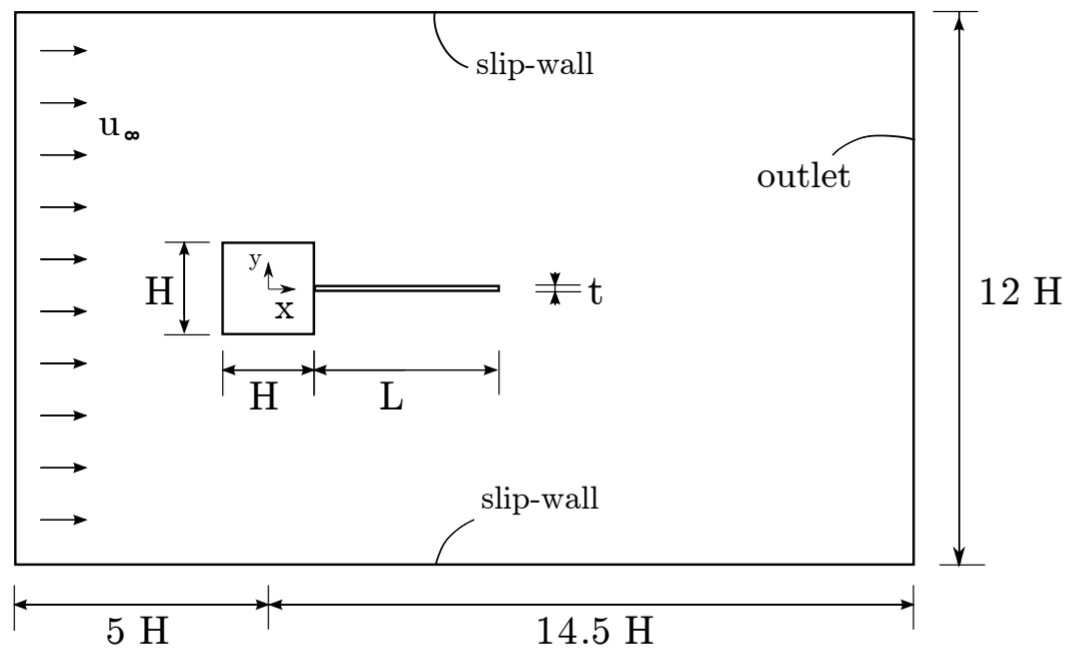
\includegraphics[width=\linewidth, trim=0 0 0 0, clip]{images/sq-cyl/sq-cyl-domain.png}
  \end{subfigure}
  \hfill
  \begin{subfigure}[t]{\textwidth}
    %\centering
    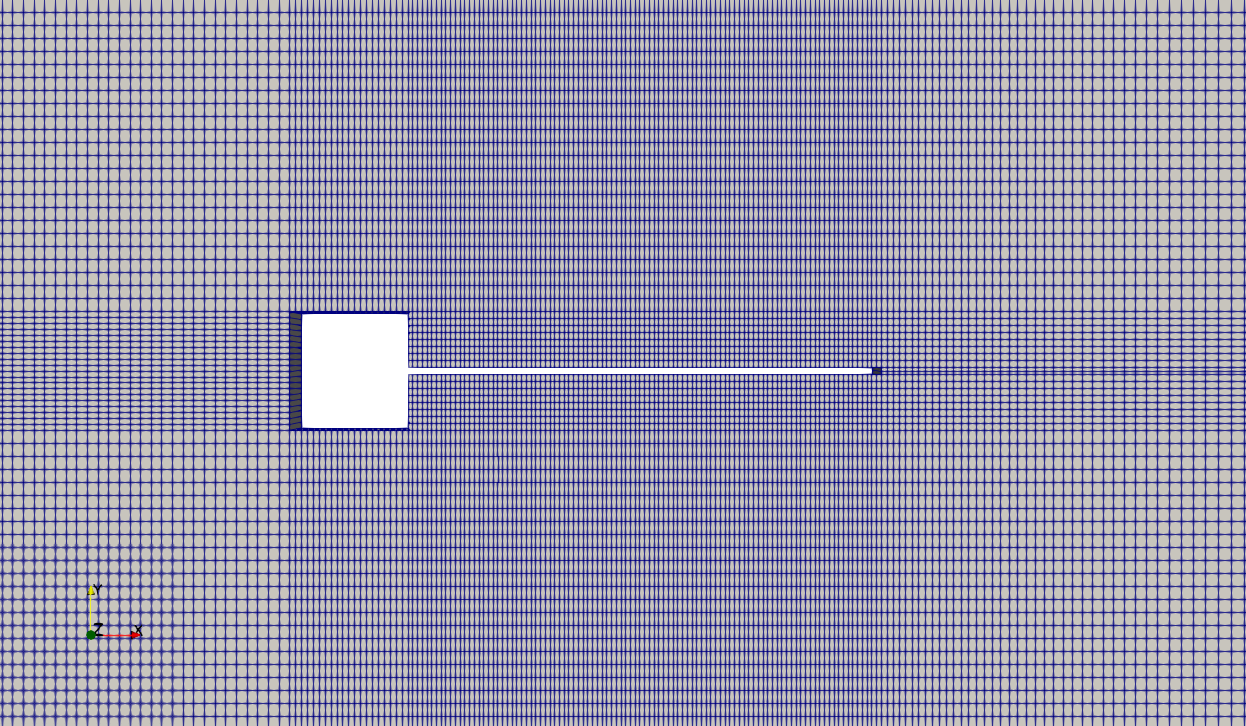
\includegraphics[width=0.86\linewidth]{images/sq-cyl/sq_mesh.png}
  \end{subfigure}
	
	
	
	
    \end{figure}
    
    \column{0.4\textwidth}
    	\scriptsize
		\begin{tabular}{ c | r } 
			symbol & value [\si{mm}]  \\ 
			\hline
			H & $10$     \\
			L & $40$  \\
			t & $0.6$  \\			
		\end{tabular}

		\vspace{1.5cm}
		\begin{tabular}{ l c  | c } 
			\multicolumn{2}{c|}{parameter} & value  \\ 
			\hline
			$\rho_F$ & \si{kg.m^{-3}} & \cellcolor{blue!20} $1.18$   \\
			$\mu$& \si{kg.m^{-1}.s^{-1}} & \cellcolor{blue!20} $1.82 \cdot 10^{-5}$  \\
			Re &  & \cellcolor{blue!20} $332$ \\
			$\vec{u}_{\infty}$ & \si{m.s^{-1}} & \cellcolor{blue!20} $0.513$ \\
			flow & & \cellcolor{blue!20} laminar \\
			\hline
			$\rho_S$ & \si{kg.m^{-3}} & \cellcolor{orange!50} 100    \\
			E & \si{Pa} & \cellcolor{orange!50} $2.5\cdot 10^5$    \\
			\hline
			$M$ & & $ \cellcolor{green!10} 1.18\cdot 10^{-2}$     \\
			\hline
			$U_R$ & & $ \approx 1\cdot 10^{-2}$  \\
			$C_Y$ & & $  1.24 \cdot 10^{-6}$  \\			

		\end{tabular}
\end{columns}
\end{frame}



\begin{frame}{Square Bluff Body: simulation}

\begin{columns}

\column{0.5\textwidth}    

\begin{figure}[t]
\vspace*{-0.8cm}
\centering % <-- added
\begin{subfigure}{0.5\textwidth}
  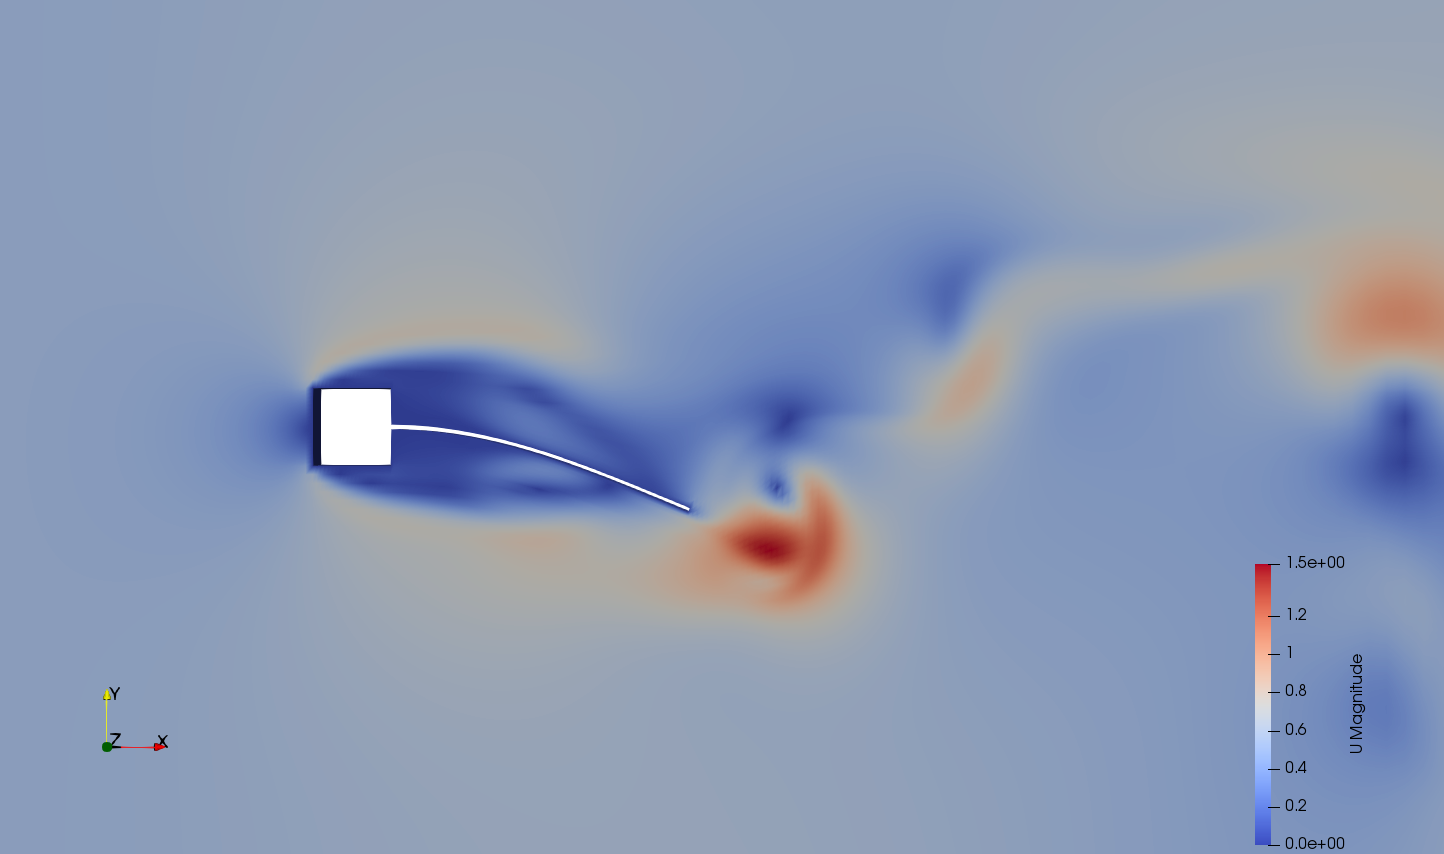
\includegraphics[width=\linewidth]{images/sq-cyl/sq_v1.png}
  \caption{t=3.37s velocity}
\end{subfigure}\hfil % <-- added
\begin{subfigure}{0.5\textwidth}
  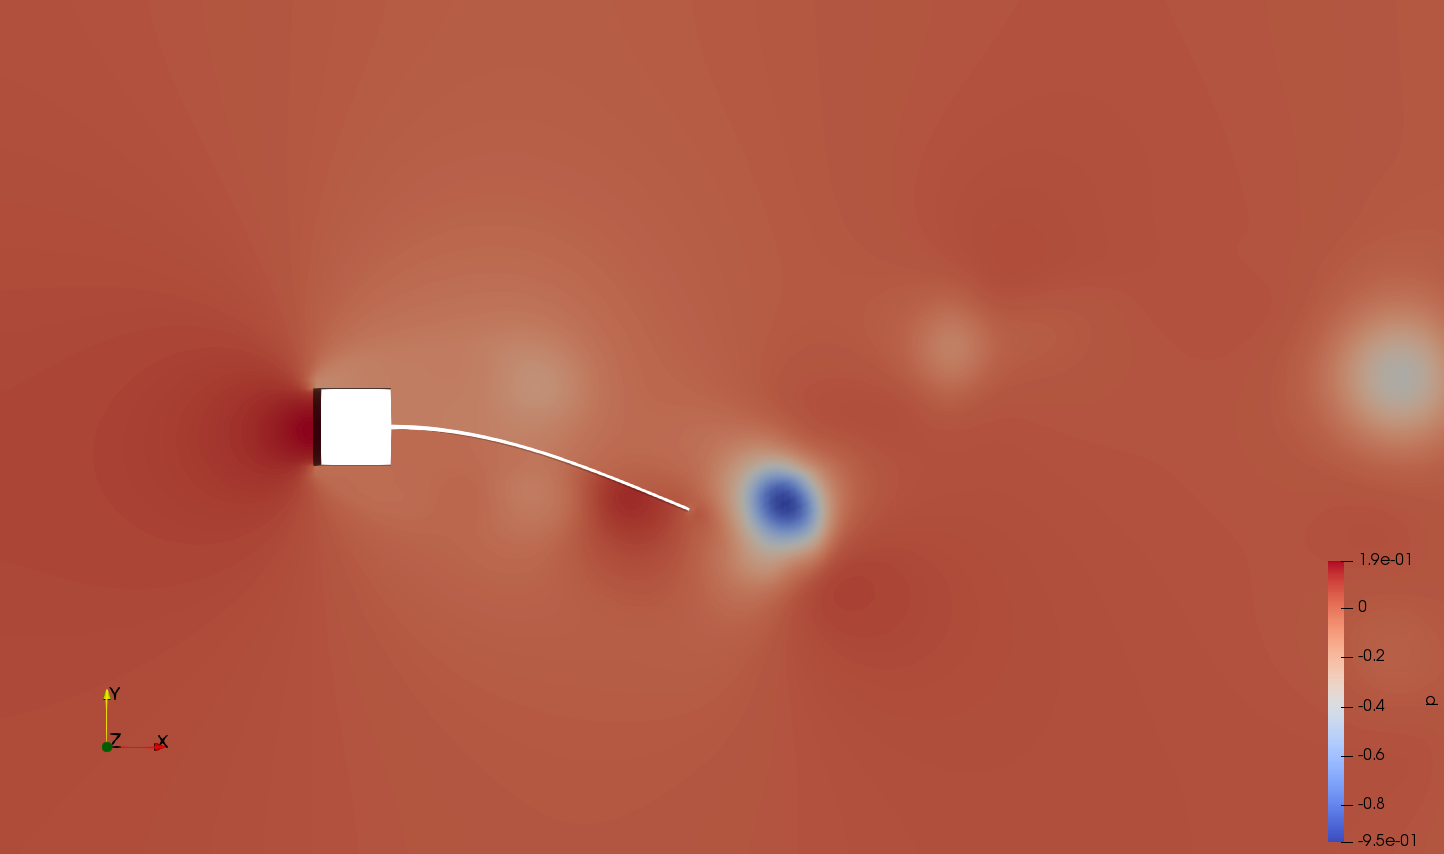
\includegraphics[width=\linewidth]{images/sq-cyl/sq_p1.png}
  \caption{t=3.37s pressure}
\end{subfigure}\hfil % <-- added

\medskip
\begin{subfigure}{0.5\textwidth}
  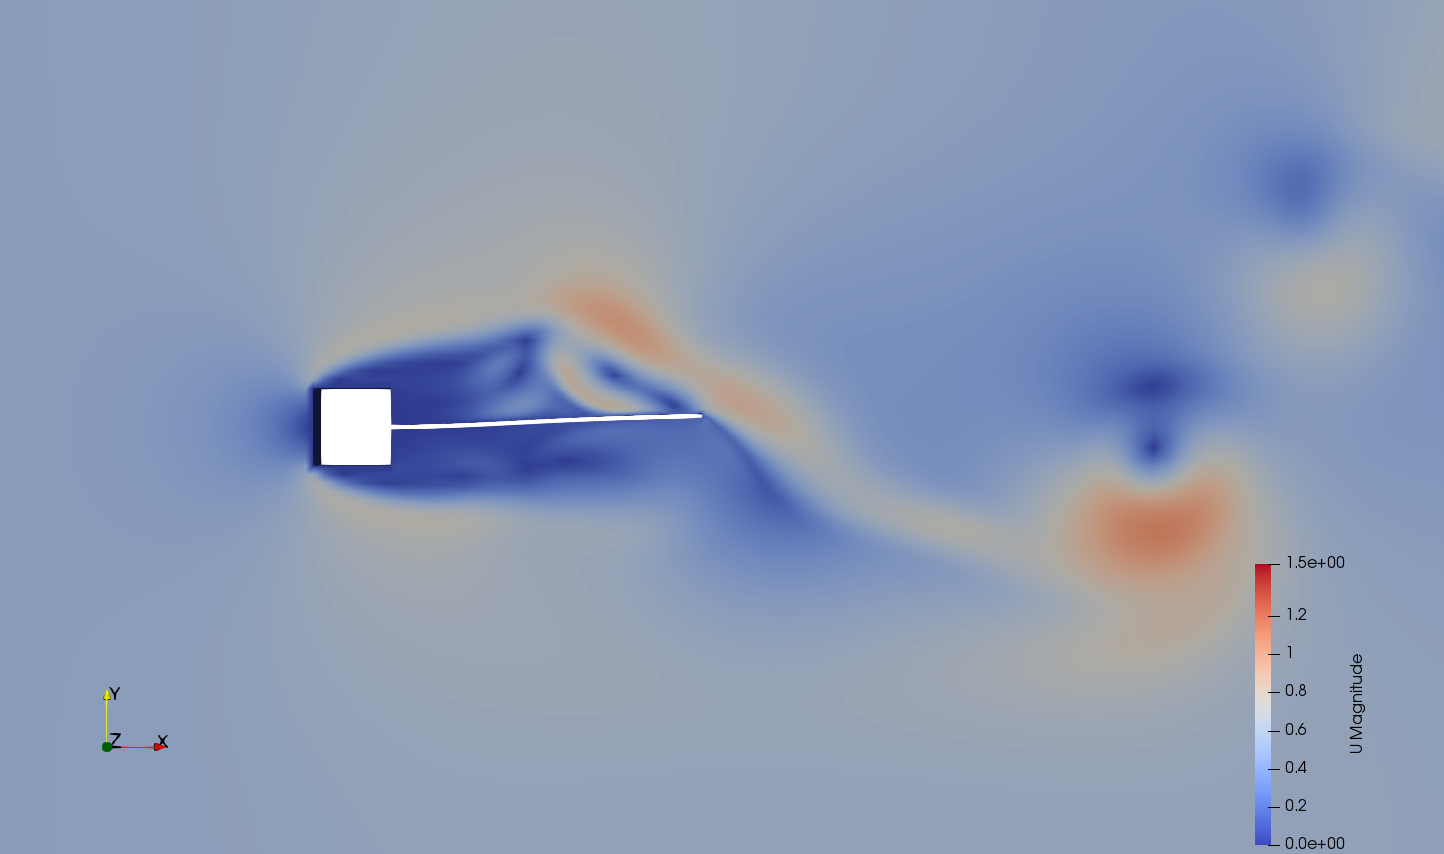
\includegraphics[width=\linewidth]{images/sq-cyl/sq_v2.png}
  \caption{t=3.47s velocity}
  \label{fig:sq_v2}
\end{subfigure}\hfil % <-- added
\begin{subfigure}{0.5\textwidth}
  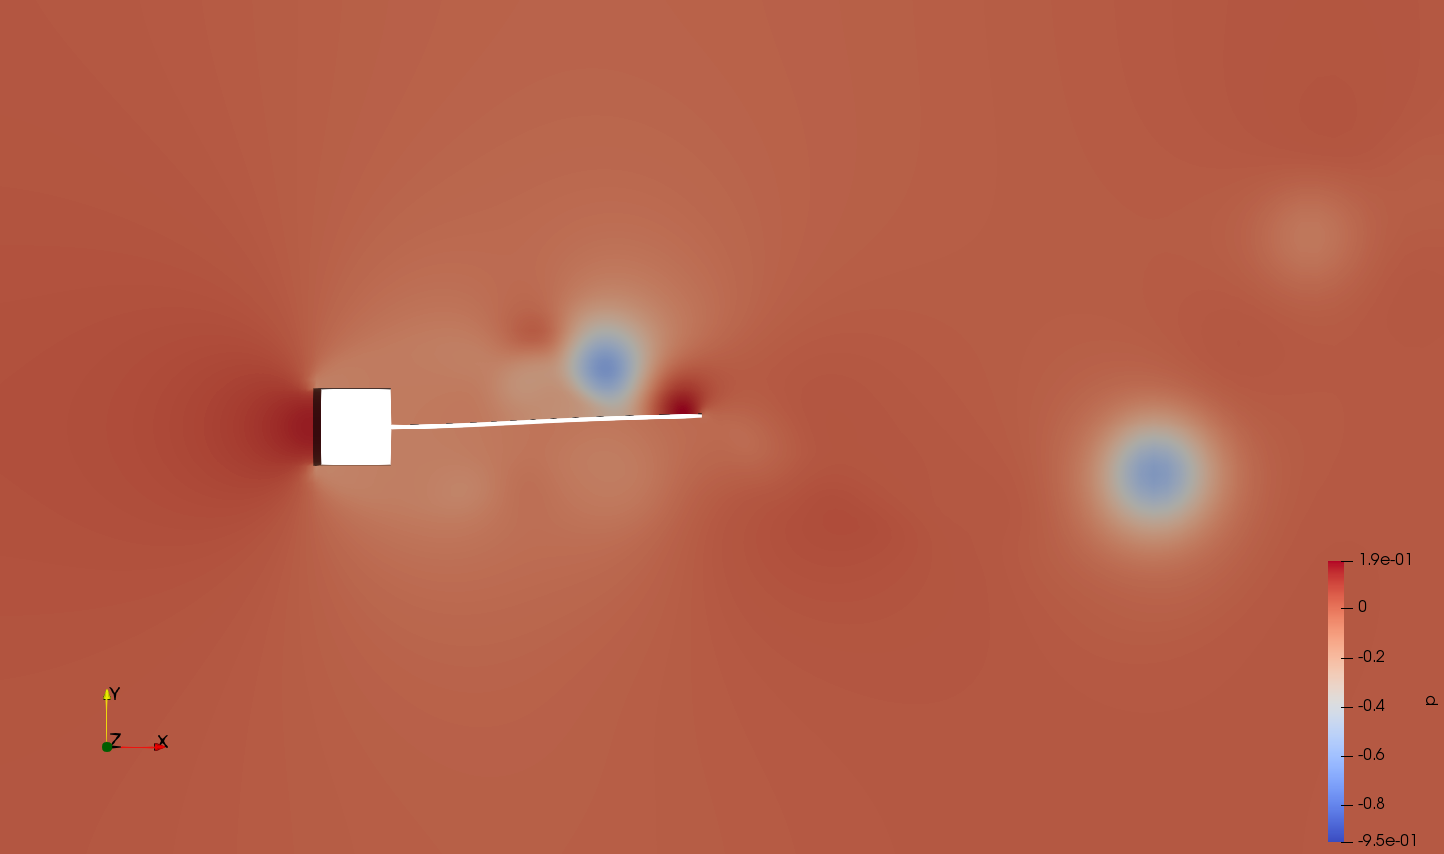
\includegraphics[width=\linewidth]{images/sq-cyl/sq_p2.png}
  \caption{t=3.47s pressure}
  \label{fig:sq_p2}
\end{subfigure}\hfil % <-- added

\begin{subfigure}{0.5\textwidth}
  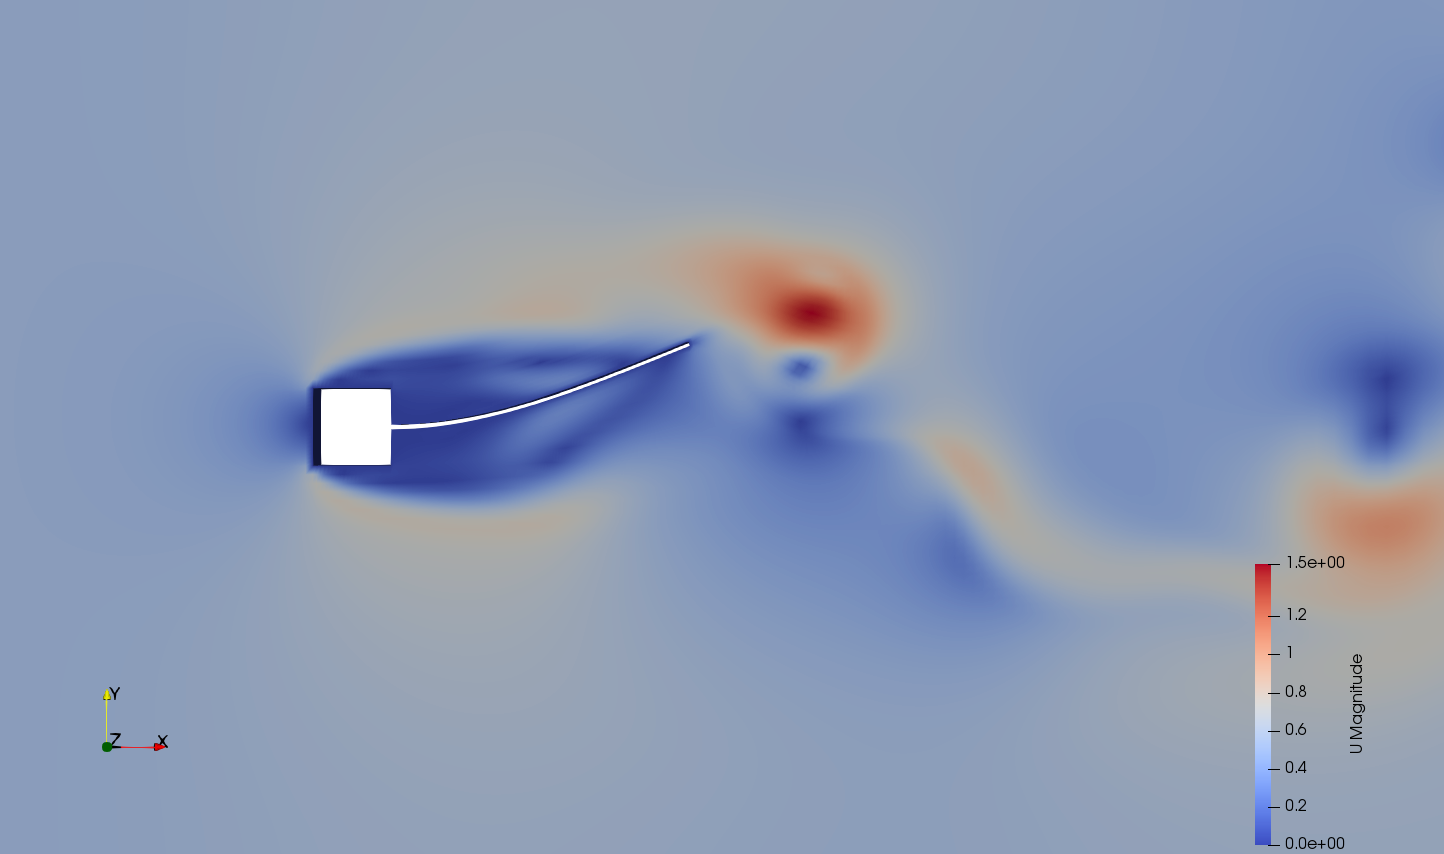
\includegraphics[width=\linewidth]{images/sq-cyl/sq_v3.png}
  \caption{t=3.53s velocity}
\end{subfigure}\hfil % <-- added
\begin{subfigure}{0.5\textwidth}
  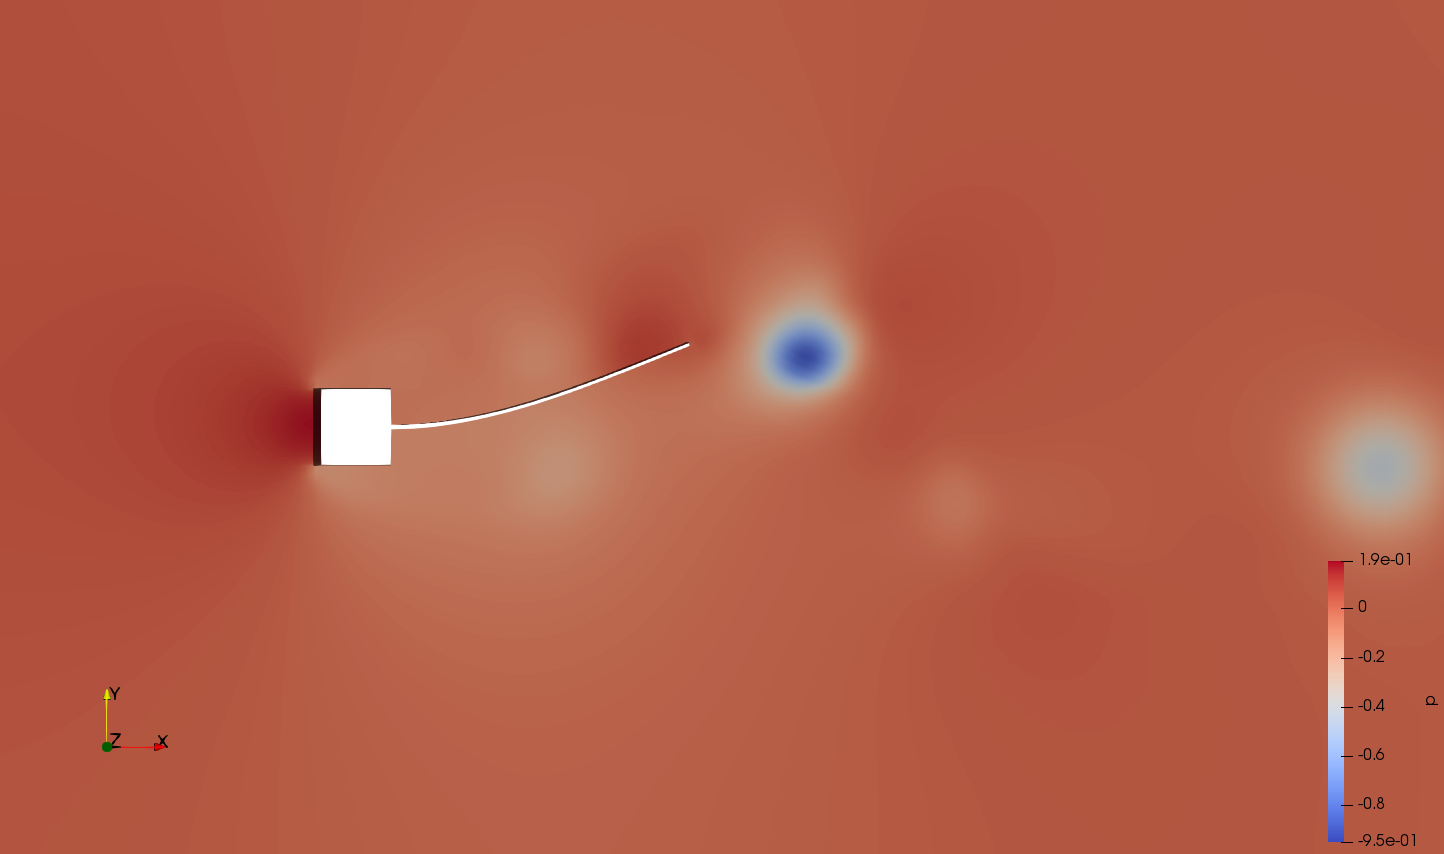
\includegraphics[width=\linewidth]{images/sq-cyl/sq_p3.png}
  \caption{t=3.53s pressure}
\end{subfigure}\hfil % <-- added

\end{figure}

\column{0.5\textwidth}

\footnotesize
\begin{itemize}
    \itemsep 10pt
    \item \textbf{MBDyn} model: 10 \texttt{beam3} elements
    \item \textbf{OpenFOAM} model: \texttt{pimpleFOAM}
    \begin{itemize}
        \item $\approx 29k$ \texttt{hex} cells
    \end{itemize}
    \item \textbf{preCICE} configuration:
    \begin{itemize}
        \item serial implicit coupling
        \item mapping: RBF
        \item acceleration: IQN-ILS
    \end{itemize}
    %\pause
    \item \textbf{performance}
    \begin{itemize}
        \item 8 avg. iterations to converge
    \end{itemize}

\end{itemize}

\end{columns}

\end{frame}

\begin{frame}{Square Bluff Body: results}

comparison made on \textbf{vertical tip displacement}

\vspace{0.8cm}

\begin{columns}



\column{0.5\textwidth}

\begin{figure}[htbp!]
    \vspace{-2.2cm}
	\centering
	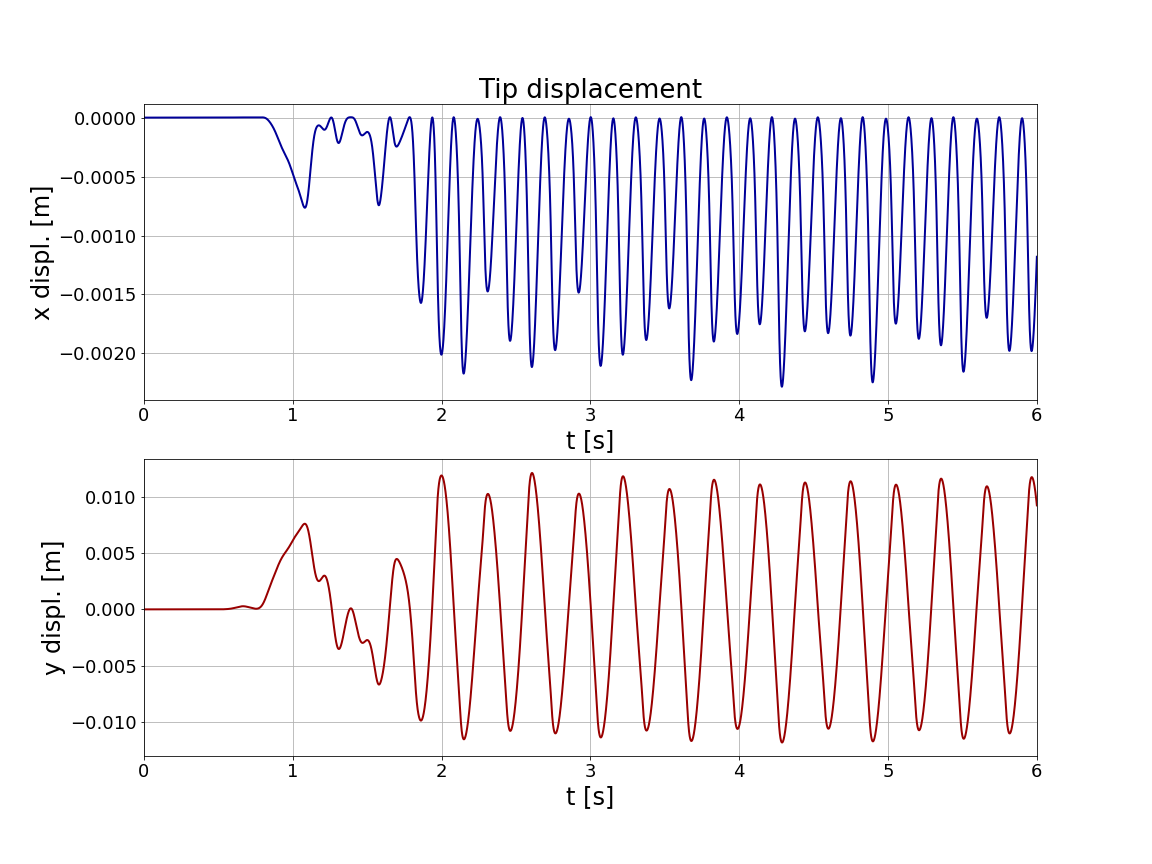
\includegraphics[width=0.98\textwidth, trim=20 20 20 50, clip]{images/sq-cyl/disp_sq_pres.png}
	%\caption{tip displacement}
\end{figure}

\column{0.5\textwidth}
\scriptsize
		\begin{tabular}{ l | c  c } 
			Study & $f$ [Hz] & $d_{y}$ [mm]   \\ 
			\hline
            Wall and Ramm & $3.08$ & $13.1$ \\
            Kassiotis et al.& $2.98$ & $10.5$ \\
            Wood et al. & $2.94$ & $11.5$ \\
            Olivier et al. & $3.17$ & $9.5$ \\
            Walhorn et al. & $3.14$ & $10.2$ \\
            Matthies and Steindorf  & $3.13$ & $11.8$ \\ 
            Dettmer and Peric & $3.03$ & $12.5$ \\
            Habchi et al. & $3.25$ & $10.2$ \\
            Froehle and Persson  & $3.18$ & $11.2$ \\
            Sanchez et al. & $3.15$ & $11.5$ \\
            \hline
            \cellcolor{green!10}average &\cellcolor{green!10} $3.1$ &\cellcolor{green!10} $11.2$\\
            \cellcolor{green!10}std. dev. &\cellcolor{green!10} $\pm0.09$ &\cellcolor{green!10} $\pm1.06$\\ 
            \hline
            Present study    & $3.067$ & $11.2$ \\
            
		\end{tabular}


\end{columns}

\end{frame}




\begin{frame}{Turek-Hron FSI2 Benchmark (turek et. al 2006): domain}


\begin{columns}
    \column{0.6\textwidth}
    \begin{figure}[t]
    \vspace*{-1.5cm}
    \hspace*{-0.2cm}
	\centering
	  \begin{subfigure}[t]{\textwidth}
    \centering
    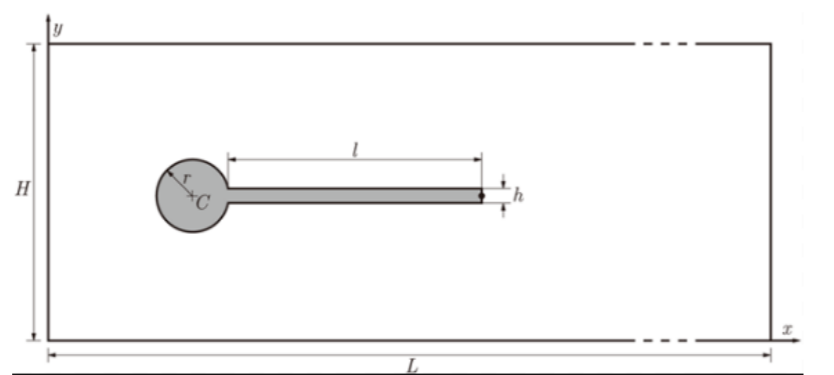
\includegraphics[width=0.865\textwidth, trim=0 0 50 0, clip]{images/FSI2/FSI2.png}
  \end{subfigure}
  \begin{subfigure}[t]{\textwidth}
    %\centering
    \hspace{3pt}
    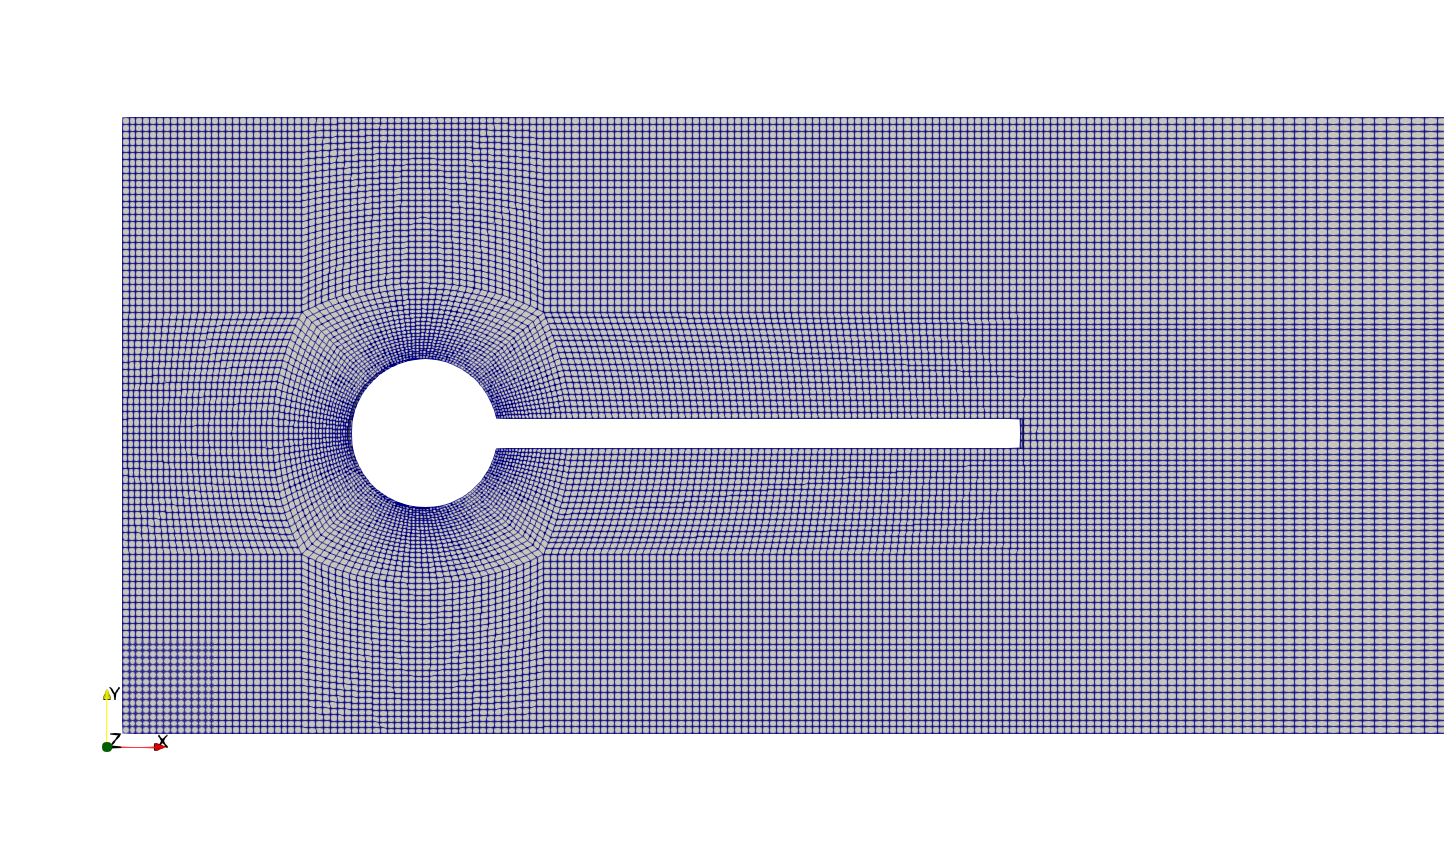
\includegraphics[width=0.89\textwidth]{images/FSI2/FSI2-mesh.png}
  \end{subfigure}
	
	
	
	
    \end{figure}
    
    \column{0.4\textwidth}
    	\scriptsize
		\begin{tabular}{ c | r } 
			symbol & value [m]  \\
			\hline
			H  & $0.41$     \\
			L  & $2.5$  \\
			l  & $0.35$  \\
			h  & $0.02$  \\
			C  & $\left(0.2,0.2 \right)$  \\
			r  & $0.05$  \\
			\end{tabular}

		\vspace{0.5cm}
		\begin{tabular}{ l c  | c } 
			\multicolumn{2}{c|}{parameter} & value  \\ 
			\hline
			$\rho_F$ & \si{kg.m^{-3}} & \cellcolor{blue!20} $1000$   \\
			$\nu$& \si{m^2.s^{-1}} & \cellcolor{blue!20} $1 \cdot 10^{-3}$  \\
			Re &  & \cellcolor{blue!20} $100$ \\
			$\vec{u}_{max}$ & \si{m.s^{-1}} & \cellcolor{blue!20} $1.5$ \\
			$\bar{u}$ & \si{m.s^{-1}} & \cellcolor{blue!20} $1$ \\
			flow & & \cellcolor{blue!20} laminar \\
			\hline
			$\rho_S$ & \si{kg.m^{-3}} & \cellcolor{orange!50} $10000$    \\
			E & \si{Pa} & \cellcolor{orange!50} $1.4\cdot 10^6$    \\
			\hline
			$M$ & & $ \cellcolor{green!10} 0.1$     \\
			\hline
			$U_R$ & & $ 8.45\cdot 10^{-2}$  \\
			$C_Y$ & & $  7.14 \cdot 10^{-4}$  \\			

		\end{tabular}
\end{columns}


    
\end{frame}



\begin{frame}{Turek-Hron FSI2 Benchmark: simulation}

\begin{columns}

\column{0.5\textwidth}    

\begin{figure}[htb]
\vspace*{-0.8cm}
\centering % <-- added
\begin{subfigure}{0.5\textwidth}
  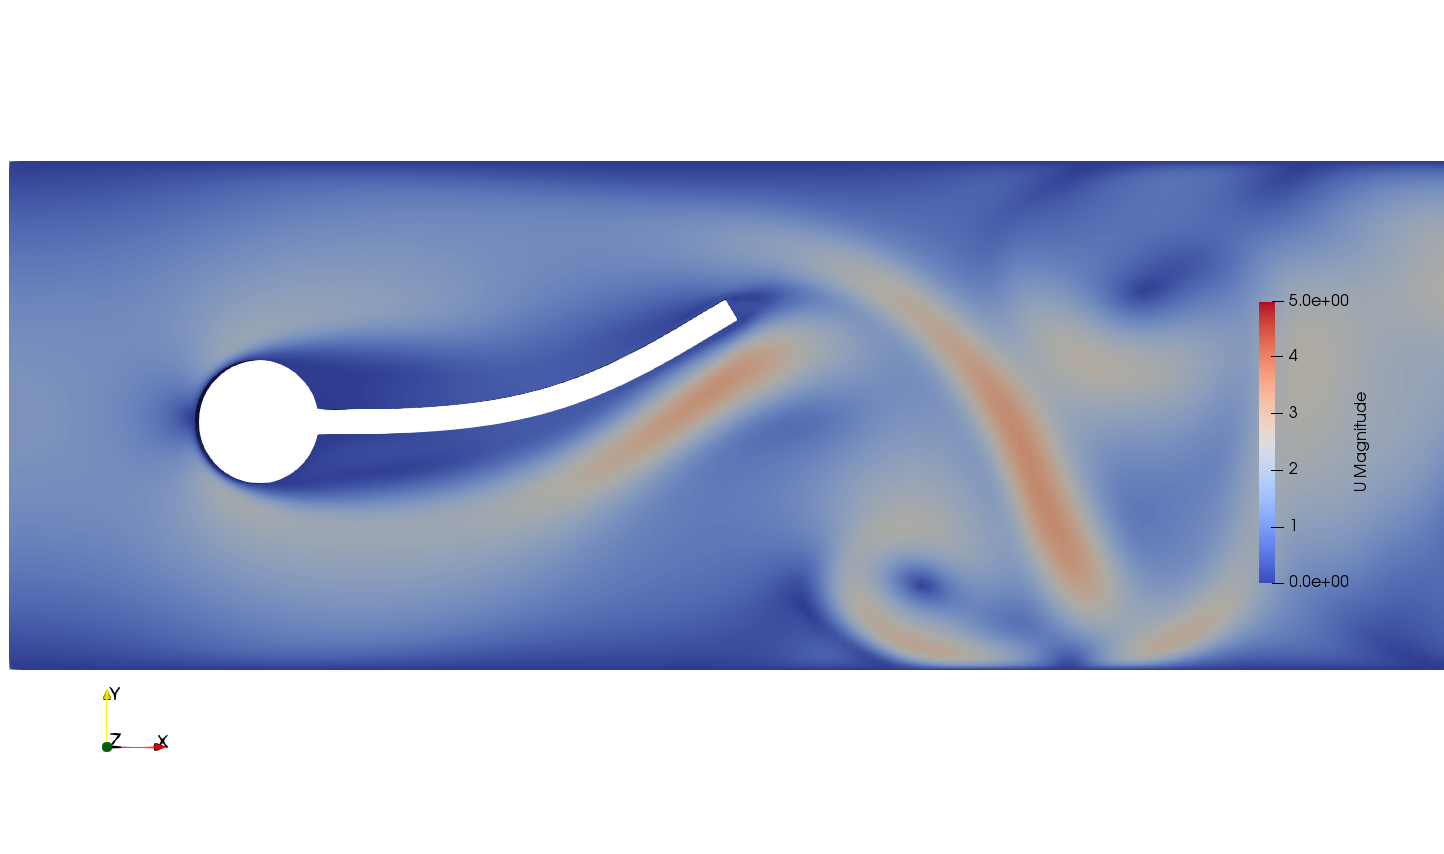
\includegraphics[width=\linewidth, trim=0 120 0 120, clip]{images/FSI2/fsi2_v1.png}
  \caption{t=5.0s velocity}
  \label{fig:fsi2_v1}
\end{subfigure}\hfil % <-- added
\begin{subfigure}{0.5\textwidth}
  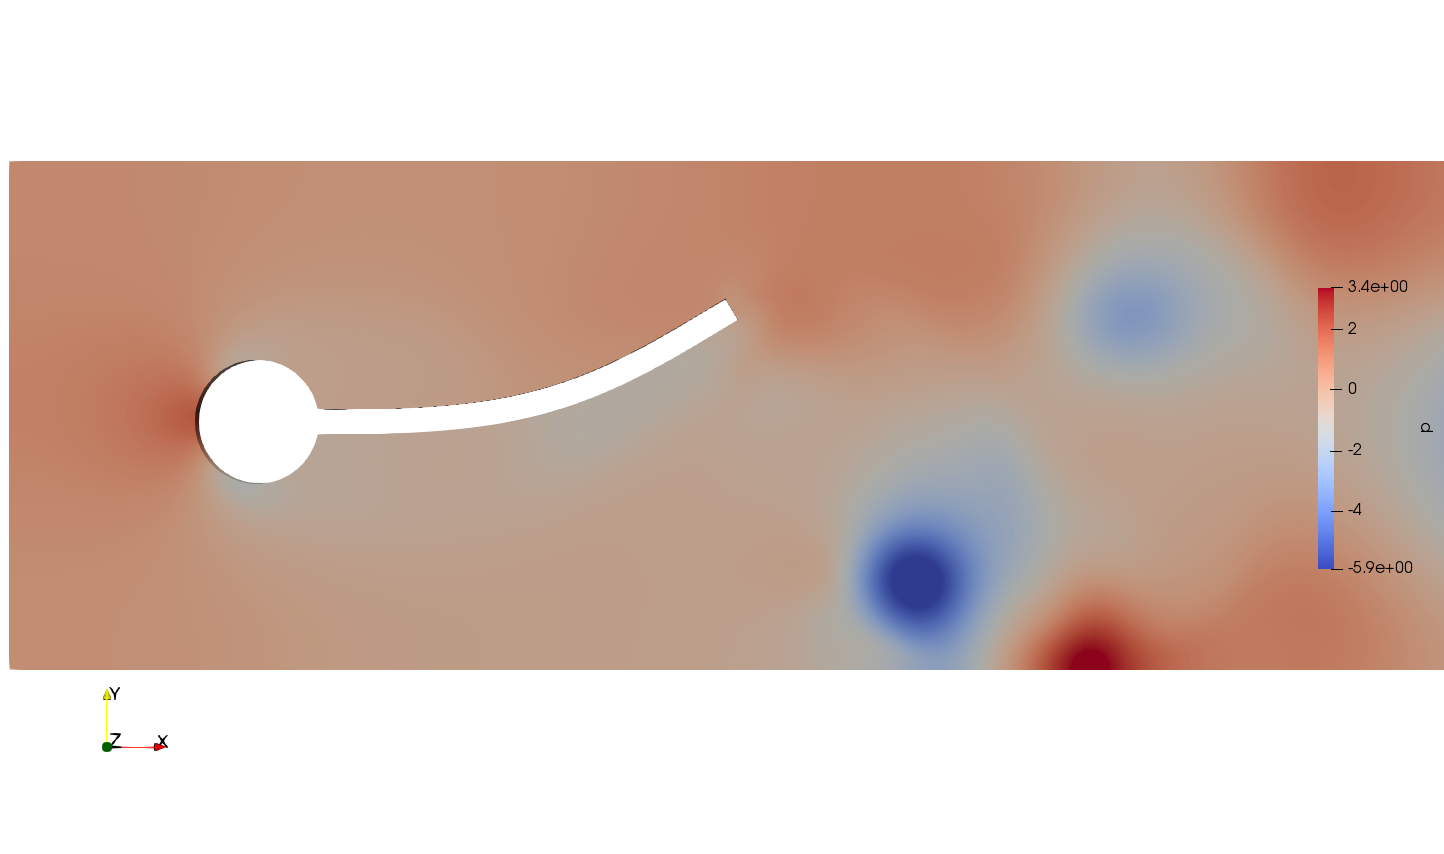
\includegraphics[width=\linewidth, trim=0 120 0 120, clip]{images/FSI2/fsi2_p1.png}
  \caption{t=5.0s pressure}
  \label{fig:fsi2_p1}
\end{subfigure}\hfil % <-- added

\medskip

\begin{subfigure}{0.5\textwidth}
  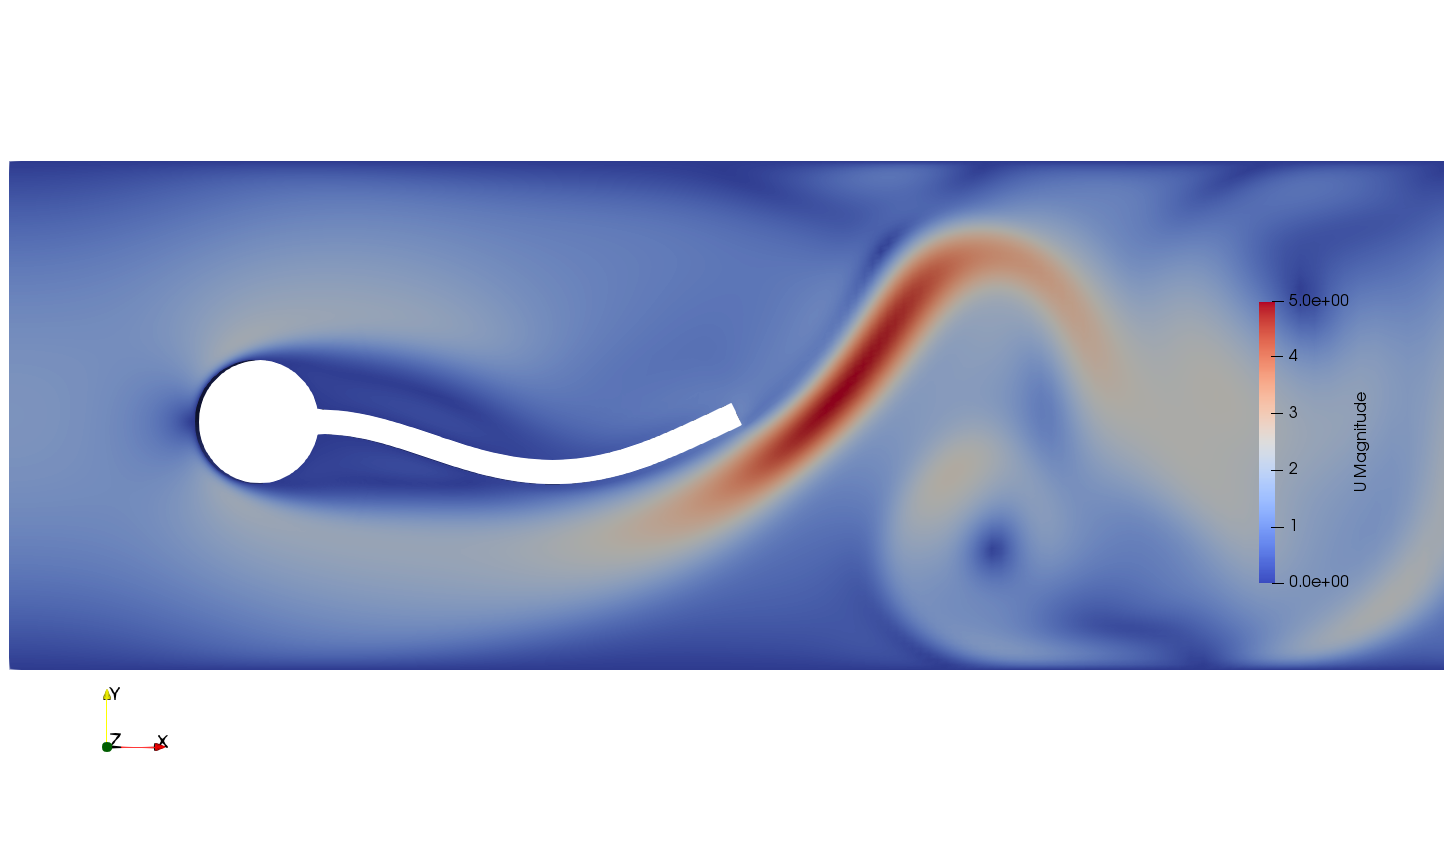
\includegraphics[width=\linewidth, trim=0 120 0 120, clip]{images/FSI2/fsi2_v2.png}
  \caption{t=5.135s velocity}
  \label{fig:fsi2_v2}
\end{subfigure}\hfil % <-- added
\begin{subfigure}{0.5\textwidth}
  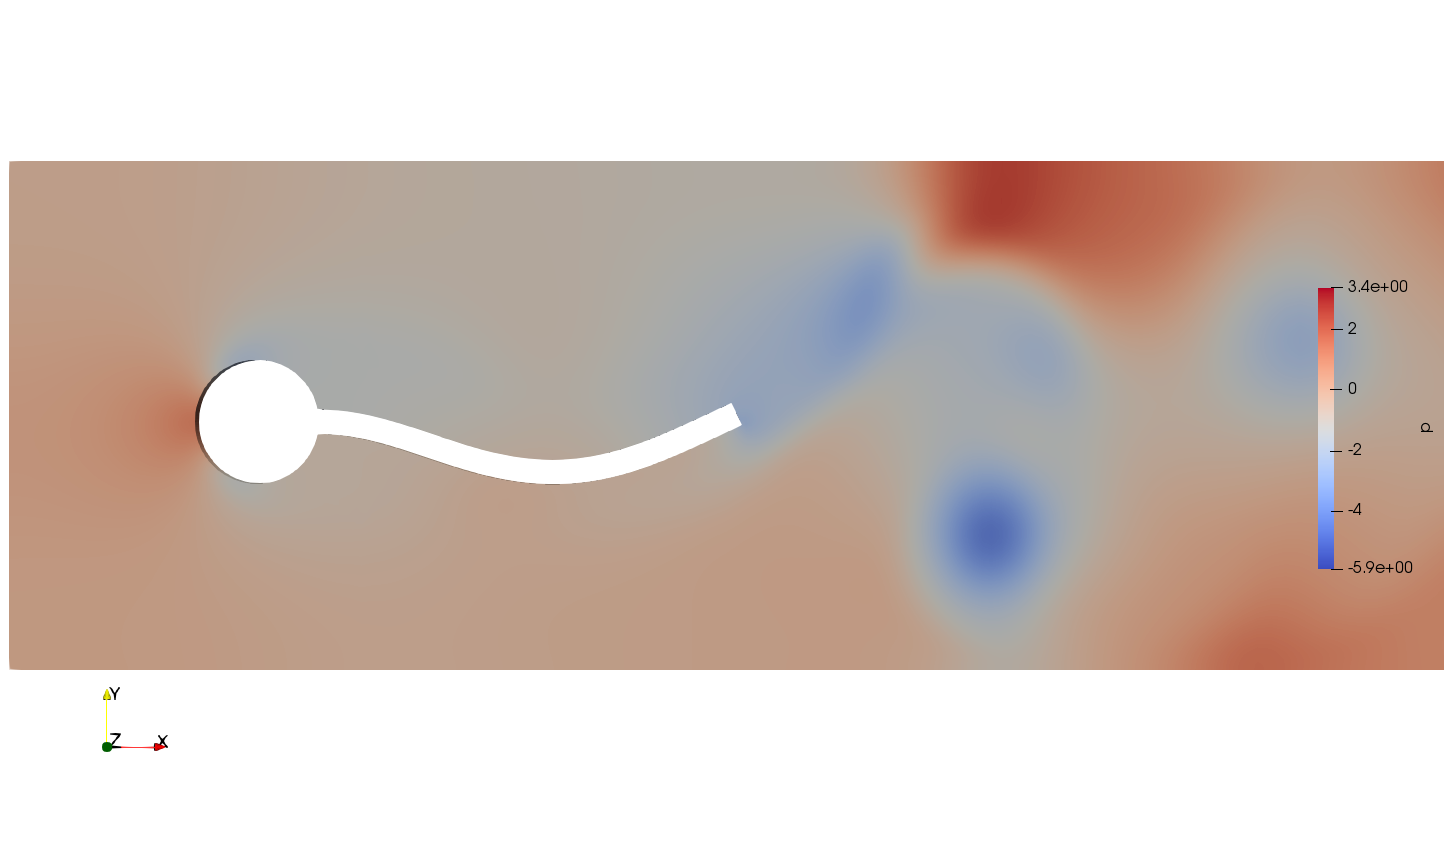
\includegraphics[width=\linewidth, trim=0 120 0 120, clip]{images/FSI2/fsi2_p2.png}
  \caption{t=5.135s pressure}
  \label{fig:fsi2_p2}
\end{subfigure}\hfil % <-- added

\medskip

\begin{subfigure}{0.5\textwidth}
  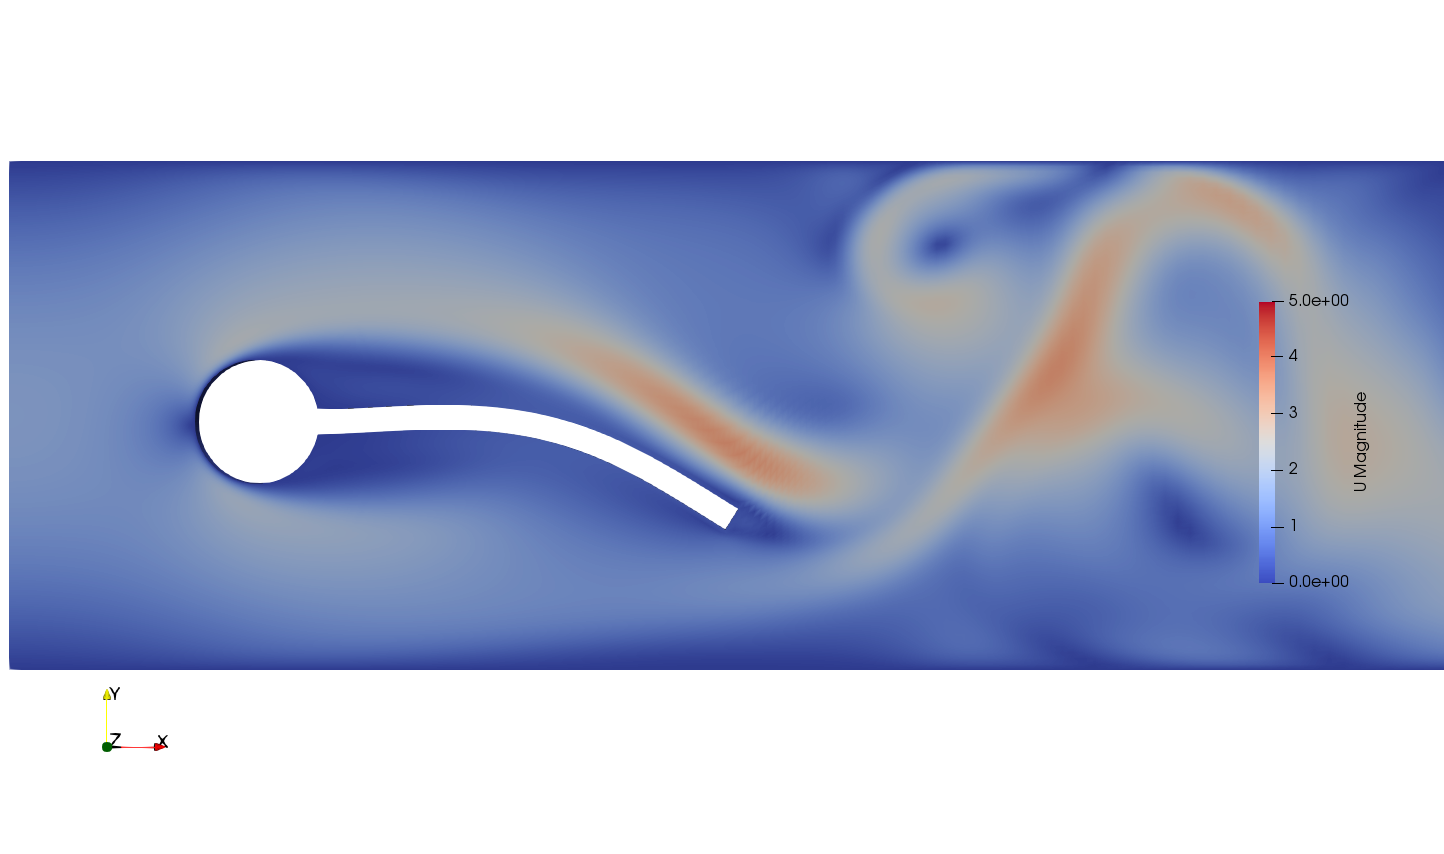
\includegraphics[width=\linewidth, trim=0 120 0 120, clip]{images/FSI2/fsi2_v3.png}
  \caption{t=5.27s velocity}
  \label{fig:fsi2_v3}
\end{subfigure}\hfil % <-- added
\begin{subfigure}{0.5\textwidth}
  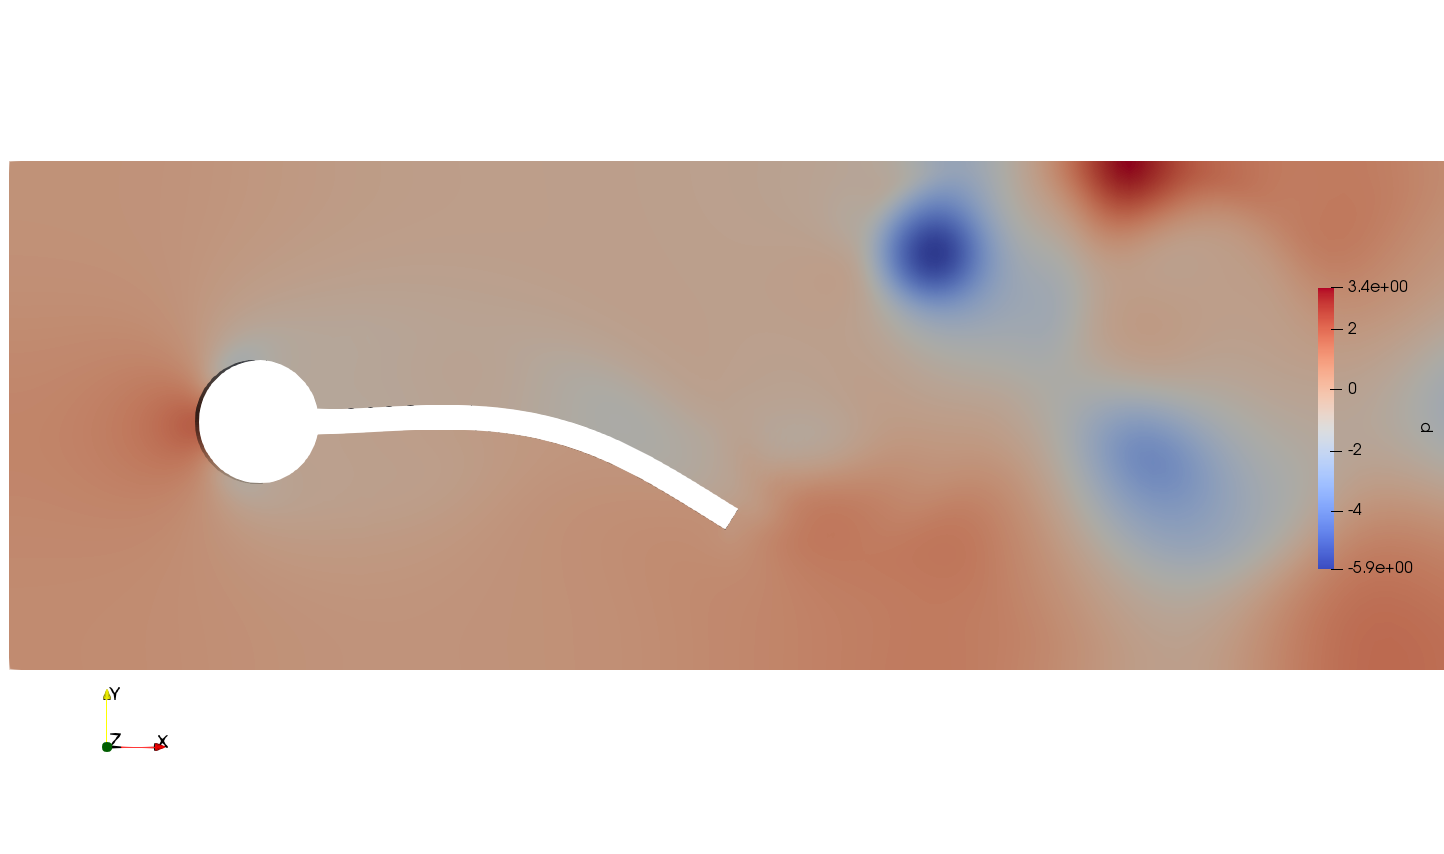
\includegraphics[width=\linewidth, trim=0 120 0 120, clip]{images/FSI2/fsi2_p3.png}
  \caption{t=5.27s pressure}
  \label{fig:fsi2_p3}
\end{subfigure}\hfil % <-- added

%\caption{FSI2: fluid solution}
\label{fig:FSI2_sol}
\end{figure}

\column{0.5\textwidth}

\footnotesize
\begin{itemize}
    \itemsep 10pt
    \item \textbf{MBDyn} model: 10 \texttt{beam3} elements
    \item \textbf{OpenFOAM} model: \texttt{pimpleFOAM}
    \begin{itemize}
        \item $\approx 25k$ \texttt{hex} cells
    \end{itemize}
    \item \textbf{preCICE} configuration:
    \begin{itemize}
        \item serial implicit coupling
        \item mapping: RBF
        \item acceleration: IQN-ILS
    \end{itemize}
    %\pause
    \item \textbf{performance}
    \begin{itemize}
        \item 14.5 avg. iterations to converge
    \end{itemize}
\end{itemize}

\end{columns}

\end{frame}


\begin{frame}{Turek-Hron FSI2 Benchmark: results}

\begin{columns}

\column{0.3\textwidth}
%\vspace{1cm}
comparison made on \\ \textbf{tip displacements}:

\column{0.7\textwidth}


\vspace{-1cm}
\begin{figure}[htbp!]
    %\vspace{-1.8cm}
	%\centering
	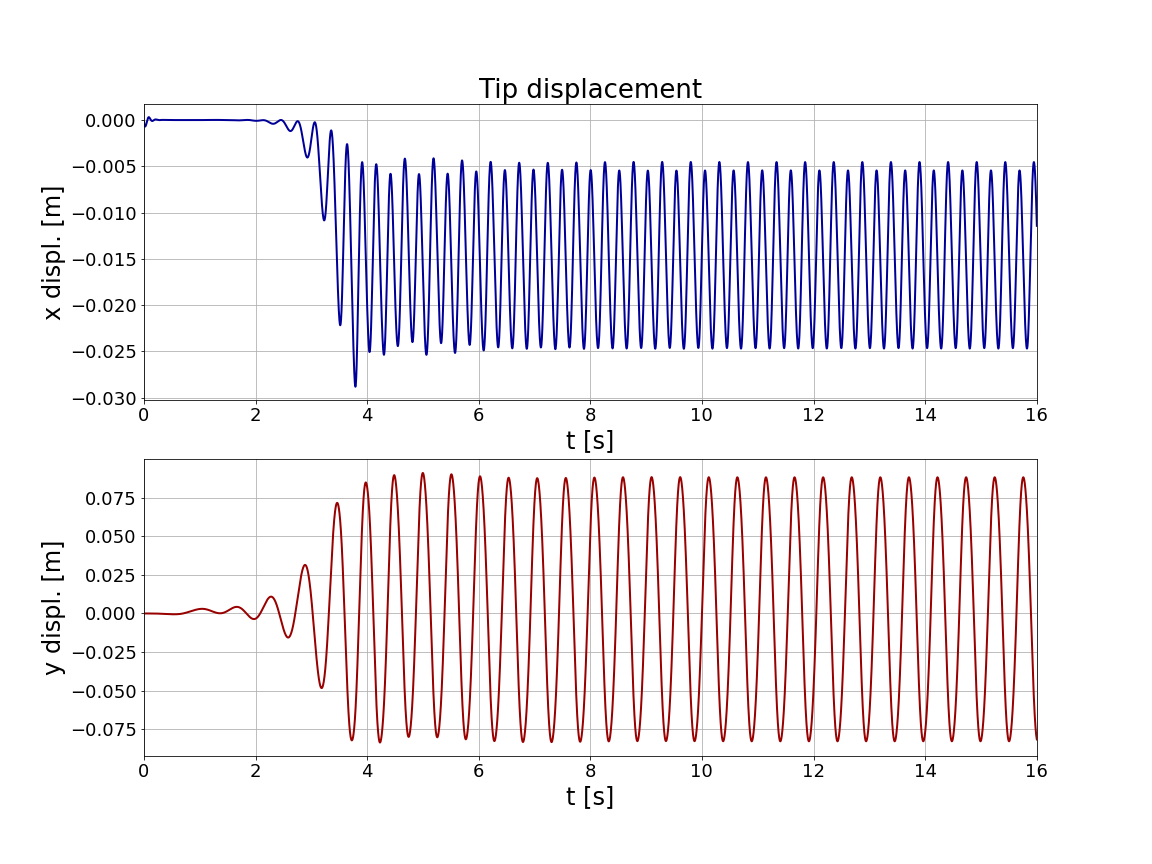
\includegraphics[width=0.9\textwidth, trim=20 20 20 20, clip]{images/FSI2/disp_fsi2_pres.png}
\end{figure}


\end{columns}





\footnotesize
\begin{center}
\begin{tabular}{ l | c c | c c  |  } 
	Study & $d_{x\,tip}$ [\si{mm}] & f [\si{Hz}] & $d_{y\,tip}$ [\si{mm}] & f [\si{Hz}] \\ 
	\hline
	\hline
	Benchmark & $-14.58\pm12.44$ & $3.8$ & $1.23\pm80.6$ & $2.0$ \\
	Turek et al. (2010) & $-14.85\pm12.70$ & $3.86$ & $1.30\pm81.7$ & $1.93$ \\
	Gjertsen & $-14.83\pm13.11$ & & $1.24\pm81.6$ & \\
	Degroote & $-14.07\pm12.37$ & $3.7$ & $1.18\pm76.5$ & $1.9$ \\
	\hline
	Present study & $-14.95\pm9.85$ & $3.87$ & $2.78\pm83.39$ & $1.93$ \\ 
\end{tabular}
    
\end{center}
\vspace{0.2cm}
% Axial flexibility of beams?

\end{frame}




\begin{frame}{Turek-Hron FSI3 Benchmark}

\footnotesize
\begin{center}
\begin{tabular}{ l c l | c | c } 
	\multicolumn{3}{c|}{parameter} & FSI2 & FSI3   \\ 
	\hline
	solid density  &  $\rho$ & \si{kg.m^{-3}} & $10000$ & $1000$     \\
	Elastic modulus  & E & \si{Pa} & $1.4\cdot 10^6$ & $5.6\cdot 10^6$   \\
	max flow velocity & $\vec{u}_{max}$ & \si{m.s^{-1}} & $1.5$ & $3$ \\
	mean flow velocity & $\vec{u}$ & \si{m.s^{-1}} & $1$ & $2$  \\
    \hline
    mass number  &  $M$ & & \cellcolor{red!10} $0.1$ & \cellcolor{red!10} $1$     \\
	reduced velocity & $U_R$ & & $8.45 \cdot 10^{-2}$  & $2.67\cdot 10^{-2}$  \\
	Cauchy number  & $C_Y$ & & \cellcolor{yellow!25}  $7.14\cdot 10^{-4}$  & \cellcolor{yellow!25} $7.14\cdot 10^{-4}$  \\
	Reynolds number & $Re$ & & $100$ & $200$ \\
\end{tabular}    
\end{center}
\normalsize
\vspace{0.5cm}
Despite acting on:
\begin{itemize}
    \item \textcolor{pblue}{fluid domain}: mesh, convergence...
    \item \textcolor{dorange}{solid domain}: number of elements, solver...
    \item \textcolor{teal}{coupling}: convergence, timestep extrapolation, filtering...
\end{itemize}
\vspace{0.5cm}
\large
At present time this setup \textcolor{red}{does not converge}
    
\end{frame}

\begin{frame}{Turek-Hron FSI3 Benchmark}
\label{fsi2}
\textbf{Sensitivity analysis}: change $\rho_F$ and $E$ 


\footnotesize
\begin{center}
	\begin{tabular}{ c | c | c c c c c |} 
	&  & \multicolumn{5}{c|}{mass ratio} \\
		
	$U_R$ & E \si{MPa} & 0.1 & 0.2 & 0.25 & 0.5 & 1 \\
	\hline
    $1.41\cdot 10^{-4}$ & $2\cdot 10^{5}$ & \cellcolor{green!10}2.204 & \cellcolor{green!10} & \cellcolor{green!10}2.618 & \cellcolor{green!10}3.126 & \cellcolor{green!10}4.418 \\
	$6.32\cdot 10^{-4}$ & $1\cdot 10^{4}$ & \cellcolor{green!10} & \cellcolor{green!10}15.024 & \cellcolor{green!10}43.1 & \cellcolor{red!10} & \cellcolor{red!10} \\        
	$2\cdot 10^{-3}$ & $1\cdot 10^{3}$ & \cellcolor{green!10}23.46 & \cellcolor{green!10} & \cellcolor{green!10}10.78 & \cellcolor{red!10} & \cellcolor{red!10} \\
	$6.32\cdot 10^{-3}$ & $1\cdot 10^{2}$ & \cellcolor{green!10} & \cellcolor{green!10}7.592 & \cellcolor{green!10}11.788 & \cellcolor{red!10} & \cellcolor{red!10} \\
	$1.41\cdot 10^{-2}$ & $20$ & \cellcolor{green!10}11.46 & \cellcolor{green!10} & \cellcolor{green!10}87.675 & \cellcolor{red!10} & \cellcolor{red!10} \\
	$2.67\cdot 10^{-2}$ & $5.6$ & \cellcolor{green!10}7.216 & \cellcolor{green!10}36.426 & \cellcolor{red!10} & \cellcolor{red!10} & \cellcolor{red!10}\textbf{FSI3} \\
	\hline                        
	\end{tabular}
\end{center}

\vspace{0.5cm}

\normalsize

\textbf{Observations:}
\begin{itemize}
    \item limit in \textit{mass ratio}
    \item Structural stiffness helps
    \item visible patterns in number of iterations
\end{itemize}


\hyperlink{fsi1}{\beamergotobutton{FSI1 analysis}}

\end{frame}



\section{Conclusions}

\begin{frame}{Conclusions}

%\large

\textcolor{pblue}{\textbf{Goals}}:

\begin{itemize}
    \item Exploit \textcolor{pblue}{\textbf{MBDyn}} capabilities to perform fluid-structure co-simulation
    \item Integrate \textit{MBDyn} with \textcolor{pblue}{\textbf{preCICE}} to guarantee a common interface to multiple CFD solvers
    \item validate the \textcolor{pblue}{\textbf{FSI}} simulation with the proposed setup
\end{itemize}

\pause

\vspace{0.5cm}

\textcolor{teal}{\textbf{Results}}:

\begin{itemize}
    \item the \textcolor{teal}{\textbf{adapter}} has been developed and verified
    \item Solutions comparable with \textcolor{teal}{\textbf{benchmarks}} (bluff body, FSI2...)
\end{itemize}

\pause

\vspace{0.5cm}

\textcolor{dorange}{\textbf{Open points}}:

\begin{itemize}
    \item Convergence issues when \textcolor{red}{\textit{mass ratio}} $\rightarrow 1$ 
\end{itemize}



\end{frame}

\begin{frame}{Future Development}

\textbf{Three} possible directions of further development:

\vspace{0.3cm}

\pause

\begin{enumerate}
    \item \textcolor{pblue}{\textbf{Software side}}
        \itemsep 10pt
        \begin{itemize}
            \item improve usability
            \item reduce/avoid redundancy
            \item internal optimizations (data handling, mesh topology...)
        \end{itemize}    

\pause
    
    \item \textcolor{pblue}{\textbf{Simulation side}}
    
        \begin{itemize}
            \item Reduce, possibly solve, convergence issues with \textit{mass ratio}
            \item Verify scalability, with more complex 3D cases
        \end{itemize}

\pause
    
    \item \textcolor{pblue}{\textbf{Application side}}
    
        \begin{itemize}
            \item Find further, different benchmarks (other than incompressible flow), users and cases
            \item Use or extend this setup also for \textbf{SSI} problems 
        \end{itemize}
    
\end{enumerate}


\end{frame}


\setbeamercolor{background canvas}{bg=pblue}
\begin{frame}[c,plain]{}
    \centering
    \large{\textcolor{white}{\textbf{Thank you}}}
\end{frame}


\miniframesoff

%\section*{further info}

\setbeamercolor{background canvas}{bg=white}
\begin{frame}{weak coupling}\label{couplingdetails}


  \begin{block}{staggered weak coupling}
  \begin{center}
  $
  \left\{
    \begin{aligned}
        x_f^n&=\phi_f\left(x_f^n,x_f^{n-1},x_s^{n-1} \right) \\
        x_s^n&=\phi_s\left(x_s^n,x_f^{n-1},x_s^{n} \right)
    \end{aligned}
    \right.
  $
      
  \end{center}
  \end{block}  


  \begin{block}{parallel weak coupling}
  \begin{center}
  $
  \left\{
    \begin{aligned}
        x_f^n&=\phi_f\left(x_f^n,x_f^{n-1},x_s^{n-1} \right) \\
        x_s^n&=\phi_s\left(x_s^n,x_f^{n-1},x_s^{n-1} \right)
    \end{aligned}
    \right.
  $
  \end{center}
  \end{block}  



\begin{itemize}
    \item implicit integration in time
    \item no check on convergence (no energy balance)
    \item order can be switched
\end{itemize}

\end{frame}


\begin{frame}{strong coupling}
  
  \begin{block}{staggered strong coupling}
  \begin{center}
  $
  \left\{
    \begin{aligned}
        x_f^{n,k}&=\phi_f\left(x_f^{n,k},x_f^{n,k-1},x_s^{n,k-1} \right) \\
        x_s^{n,k}&=\phi_s\left(x_s^{n,k},x_f^{n,k-1},x_s^{n,k} \right)
    \end{aligned}
    \right.
  $
      
  \end{center}
  \end{block}  

  
  \begin{block}{parallel strong coupling}
  \begin{center}
  $
  \left\{
    \begin{aligned}
        x_f^{n,k}&=\phi_f\left(x_f^{n,k},x_f^{n,k-1},x_s^{n,k-1} \right) \\
        x_s^{n,k}&=\phi_s\left(x_s^{n,k},x_f^{n,k-1},x_s^{n,k-1} \right)
    \end{aligned}
    \right.
  $
  \end{center}
  \end{block}  

\begin{itemize}
    \item implicit integration in time
    \item k iterations of the same time step up to convergence
    \item order can be switched
\end{itemize}


  \hyperlink{coupling}{\beamerreturnbutton{back}}
\end{frame}



\begin{frame}{acceleration}

  \begin{block}{fixed point equation}
  \begin{center}
  $
  \left\{
    \begin{aligned}
        x_s^n&=\phi_s  \circ \phi_f \left(x_s^n \right) \\
        x_s^n&=H \left(x_s^n \right) \\
        R(x) &=H \left(x_s^n \right) - x_s^n 
    \end{aligned}
    \right.
  $
      
  \end{center}
  \end{block}  

  \begin{block}{convergence criteria}
  \begin{center}
  absolute: $r_x^k \leq \epsilon_{abs}  \quad$  relative: $\frac{r_x^k}{x_k} \leq \epsilon_{rel} $
      
  \end{center}
  \end{block}  



\end{frame}


\begin{frame}{FPI solution}

  \begin{block}{under-relaxation}
  \begin{center}
  $x^{n,k+1} = x^{n,k} + \omega \left(H(x^{n,k}) - x^{n,k} \right)  $
      
  \end{center}
  \end{block}  
  
  \begin{itemize}
      \item $\omega$: relaxation factor
      \item constant under-relaxation
      \item Aitken
  \end{itemize}



\end{frame}


\begin{frame}{FPI solution}

  \begin{block}{Quasi-Newton}
  \begin{center}

  $
    \begin{aligned}
        R(x^k)&=r_k \\
        R(x^k) + \left. \frac{\partial R}{\partial x}\right|_{x^k} \cdot (x^{k+1} -x^k) &= 0 \\
        x^k +  \underbrace{ \left( \left. \frac{\partial R}{\partial x}\right|_{x^k}  \right)^{-1} \cdot (-r^k) }_{QN}   &=x^{k+1} 
    \end{aligned}
  $

  \end{center}
  \end{block}  
  
  \begin{itemize}
      \item approximation using residuals and data of previous iterations (and time-steps)
  \end{itemize}



\end{frame}


\begin{frame}{dimensionless numbers}
\label{dimensionless}
\begin{exampleblock}{Reduced velocity}

\begin{center}
    $U_R = \frac{V_0}{\sqrt{\frac{E}{\rho_S}}}$
\end{center}

\end{exampleblock}

\vspace{0.8cm}

\begin{itemize}
    \item ratio between the free fluid velocity and the velocity of elastic waves in a solid
    \item information on the way the two dynamics are related
    \item different orders of magnitude
\end{itemize}

\end{frame}


\begin{frame}{dimensionless numbers}

\begin{exampleblock}{Cauchy number}

\begin{center}
    $C_Y = \frac{\rho_f V_0^2}{E}$
\end{center}


\end{exampleblock}

\vspace{0.8cm}

\begin{itemize}
    \item ratio between the fluid inertial forces, quantified by the dynamic pressure, and the stiffness of the solid
    \item quantification of how much the solid is elastically deformed by the flow
\end{itemize}

\vspace{0.8cm}

\hyperlink{addedmass}{\beamerreturnbutton{back}}

\end{frame}




\begin{frame}{Mapping}
\label{mapping}
    \begin{exampleblock}{Consistent Mapping}
        \begin{figure}[htbp!]
	        \centering
		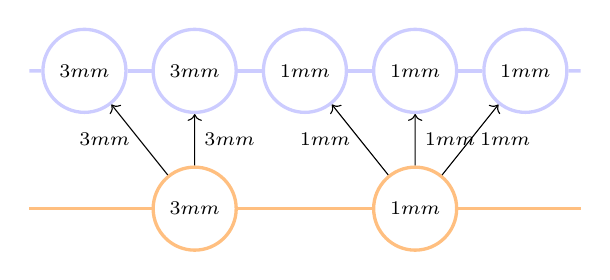
\begin{tikzpicture}[scale=0.7]
			\tikzstyle{n} = [draw, very thick, circle, minimum width=30]
			\node [n,draw=blue!20] (f1) at (1,2.5) {\scriptsize{$3mm$}};
			\node [n,draw=blue!20] (f2) at (3,2.5) {\scriptsize{$3mm$}};
			\node [n,draw=blue!20] (f3) at (5,2.5) {\scriptsize{$1mm$}};
			\node [n,draw=blue!20] (f4) at (7,2.5) {\scriptsize{$1mm$}};
			\node [n,draw=blue!20] (f5) at (9,2.5) {\scriptsize{$1mm$}};
			\node [n,draw=orange!50] (s1) at (3,0) {\scriptsize{$3mm$}};
			\node [n,draw=orange!50] (s2) at (7,0) {\scriptsize{$1mm$}};
			
			\draw [very thick, blue!20] (0,2.5) -- (f1);
			\draw [very thick, blue!20] (f1) -- (f2);
			\draw [very thick, blue!20] (f2) -- (f3);
			\draw [very thick, blue!20] (f3) -- (f4);
			\draw [very thick, blue!20] (f4) -- (f5);
			\draw [very thick, blue!20] (f5) -- (10,2.5);
			
			\draw [very thick, orange!50] (0,0) -- (s1);
			\draw [very thick, orange!50] (s1) -- (s2);
			\draw [very thick, orange!50] (s2) -- (10,0);
			
			\draw[->] (s1)-- (f1) node[midway,left] {\scriptsize{$3mm$}};
			\draw[->] (s1)-- (f2) node[midway,right] {\scriptsize{$3mm$}};
			
			\draw[->] (s2)-- (f3) node[midway,left] {\scriptsize{$1mm$}};
			\draw[->] (s2)-- (f4) node[midway,right] {\scriptsize{$1mm$}};
			\draw[->] (s2)-- (f5) node[midway,right] {\scriptsize{$1mm$}};
			
		\end{tikzpicture}
			
        \end{figure}
    \end{exampleblock}


\begin{itemize}
    \item used for \textcolor{dblue}{\textbf{displacements}}
    \item strategies:
    \begin{itemize}
        \item nearest neighbor (example above)
        \item nearest projection
        \item Radial Basis Functions
    \end{itemize}
\end{itemize}

\end{frame}


\begin{frame}{Mapping}

    \begin{exampleblock}{Conservative Mapping}
        \begin{figure}[htbp!]
	        \centering
		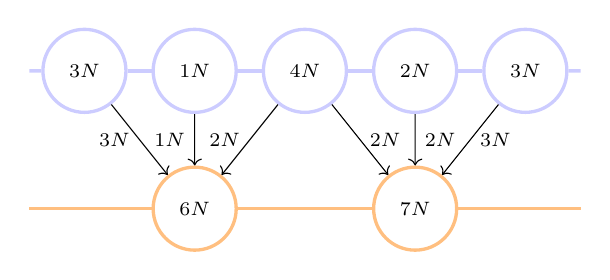
\begin{tikzpicture}[scale=0.7]
			\tikzstyle{n} = [draw, very thick, circle, minimum width=30]
			\node [n,draw=blue!20] (f1) at (1,2.5) {\scriptsize{$3N$}};
			\node [n,draw=blue!20] (f2) at (3,2.5) {\scriptsize{$1N$}};
			\node [n,draw=blue!20] (f3) at (5,2.5) {\scriptsize{$4N$}};
			\node [n,draw=blue!20] (f4) at (7,2.5) {\scriptsize{$2N$}};
			\node [n,draw=blue!20] (f5) at (9,2.5) {\scriptsize{$3N$}};
			\node [n,draw=orange!50] (s1) at (3,0) {\scriptsize{$6N$}};
			\node [n,draw=orange!50] (s2) at (7,0) {\scriptsize{$7N$}};

			\draw [very thick, blue!20] (0,2.5) -- (f1);
			\draw [very thick, blue!20] (f1) -- (f2);
			\draw [very thick, blue!20] (f2) -- (f3);
			\draw [very thick, blue!20] (f3) -- (f4);
			\draw [very thick, blue!20] (f4) -- (f5);
			\draw [very thick, blue!20] (f5) -- (10,2.5);

			\draw [very thick, orange!50] (0,0) -- (s1);
			\draw [very thick, orange!50] (s1) -- (s2);
			\draw [very thick, orange!50] (s2) -- (10,0);

			\draw[->] (f1)-- (s1) node[midway,left] {\scriptsize{$3N$}};
			\draw[->] (f2)-- (s1) node[midway,left] {\scriptsize{$1N$}};
			\draw[->] (f3)-- (s1) node[midway,left] {\scriptsize{$2N$}};
			\draw[->] (f3)-- (s2) node[midway,right] {\scriptsize{$2N$}};
			\draw[->] (f4)-- (s2) node[midway,right] {\scriptsize{$2N$}};
			\draw[->] (f5)-- (s2) node[midway,right] {\scriptsize{$3N$}};

		\end{tikzpicture}

        \end{figure}
    \end{exampleblock}


\begin{itemize}
    \item used for \textcolor{dblue}{\textbf{forces}}
    \item same strategies:
    \begin{itemize}
        \item nearest neighbor
        \item nearest projection
        \item Radial Basis Functions
    \end{itemize}
\end{itemize}

\end{frame}




\begin{frame}{Turek-Hron FSI1 Benchmark}
\label{fsi1}
\textbf{Sensitivity analysis}: change $\rho_F$ and $E$ 


\footnotesize
\begin{center}
		\begin{tabular}{ c | c | c c c c c |} 
			&  & \multicolumn{5}{c|}{mass ratio} \\
			
			$U_R$ & E[\si{MPa}] & 0.1 & 0.2 & 0.25 & 0.5 & 1 \\
			\hline
			
			$1.41\cdot 10^{-5}$ & $2\cdot 10^{5}$ & \cellcolor{green!10} & \cellcolor{green!10}2.138 & \cellcolor{green!10} & \cellcolor{green!10}2.146 & \cellcolor{green!10}3.064 \\
			$6.32\cdot 10^{-5}$ & $1\cdot 10^{4}$ & \cellcolor{green!10} & \cellcolor{green!10} & \cellcolor{green!10}2.337 & \cellcolor{red!10} & \cellcolor{red!10} \\        
			$2\cdot 10^{-4}$ & $1\cdot 10^{3}$ & \cellcolor{green!10} & \cellcolor{green!10}9.83 & \cellcolor{yellow!10} & \cellcolor{red!10} & \cellcolor{red!10} \\
			$6.32\cdot 10^{-4}$ & $1\cdot 10^{2}$ & \cellcolor{green!10}8.688 & \cellcolor{green!10} & \cellcolor{yellow!10} 24.45 & \cellcolor{red!10} & \cellcolor{red!10} \\
			$1.41\cdot 10^{-3}$ & $20$ & \cellcolor{green!10} & \cellcolor{yellow!10}18.238 & \cellcolor{yellow!10}38.398 & \cellcolor{red!10} & \cellcolor{red!10} \\
			$2.67\cdot 10^{-3}$ & $5.6$ & \cellcolor{green!10}6.314 & \cellcolor{red!10} & \cellcolor{red!10} & \cellcolor{red!10} & \cellcolor{red!10}\textbf{FSI1} \\
			\hline                        
		\end{tabular}
\end{center}

\vspace{0.5cm}

\normalsize

\textbf{Observations:}
\begin{itemize}
    \item convergence in fewer cases
    \item Structural stiffness helps
    \item visible patterns in number of iterations
\end{itemize}


\end{frame}


\begin{frame}{Turek-Hron FSI Benchmark}

\textbf{Sensitivity analysis} at $Re=1000$: change $\rho_F$ and $E$ 


\footnotesize
\begin{center}
		\begin{tabular}{ c | c | c c c c c |} 
			&  & \multicolumn{5}{c|}{mass ratio} \\
			
			$U_R$ & E[\si{MPa}] & 0.1 & 0.2 & 0.25 & 0.5 & 1 \\
			\hline
			
			$7.07\cdot 10^{-4}$ & $2\cdot 10^{5}$ & \cellcolor{green!10} & \cellcolor{green!10}5.552 & \cellcolor{green!10} & \cellcolor{green!10}6.706 & \cellcolor{green!10}8.647 \\
			$3.16\cdot 10^{-3}$ & $1\cdot 10^{4}$ & \cellcolor{green!10}10.184 & \cellcolor{green!10} & \cellcolor{green!10} & \cellcolor{green!10} & \cellcolor{green!10}9.713 \\        
			$1\cdot 10^{-2}$ & $1\cdot 10^{3}$ & \cellcolor{green!10} & \cellcolor{green!10}14.101 & \cellcolor{green!10}50.731 & \cellcolor{green!10} & \cellcolor{green!10}36.566 \\
			$3.16\cdot 10^{-2}$ & $1\cdot 10^{2}$ & \cellcolor{green!10}10.640 & \cellcolor{green!10} & \cellcolor{green!10}17.122 & \cellcolor{red!10} & \cellcolor{red!10} \\
			$7.07\cdot 10^{-2}$ & $20$ & \cellcolor{green!10} & \cellcolor{green!10}42.998 & \cellcolor{green!10}35.046 & \cellcolor{red!10} & \cellcolor{red!10} \\
			$1.34\cdot 10^{-1}$ & $5.6$ & \cellcolor{green!10}11.725 & \cellcolor{red!10} & \cellcolor{red!10} & \cellcolor{red!10} & \cellcolor{red!10} \\
			\hline                        
		\end{tabular}
	\end{center}

\vspace{0.35cm}

\normalsize

\textbf{Observations:}
\begin{itemize}
    \item broader range of convergence
    \item Structural stiffness helps
    \item visible patterns in number of iterations
\end{itemize}

\vspace{0.25cm}

\hyperlink{fsi2}{\beamerreturnbutton{back}}

\end{frame}



\begin{frame}{Interface conditions}
\label{interface}
    \begin{figure}[htbp!]
	\centering
	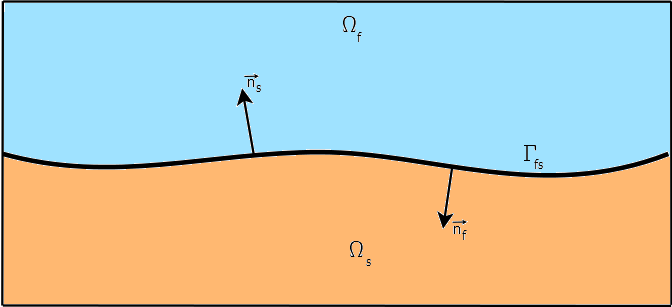
\includegraphics[width=0.65\textwidth]{images/interface}
	%\caption{fluid solid interface}
\end{figure}

\begin{itemize}
    \item \textcolor{dorange}{kinematic conditions}:
    \begin{itemize}
        \item $\Delta \vec{x}_F = \vec{u}_S$
        \item $\vec{v}_F = \frac{\partial \vec{u}_S}{\partial x}$ 
    \end{itemize}
    \item \textcolor{dblue}{equilibrium condition}:
    \begin{itemize}
        \item $\bm{\sigma_F} \cdot \hat{n}_F = \bm{\sigma_S} \cdot \hat{n}_S$
    \end{itemize}
    \end{itemize}


\end{frame}


\begin{frame}{Mesh movement}
\label{meshmotion}
    \begin{figure}

\centering
\subfloat[$t=7.0s$]{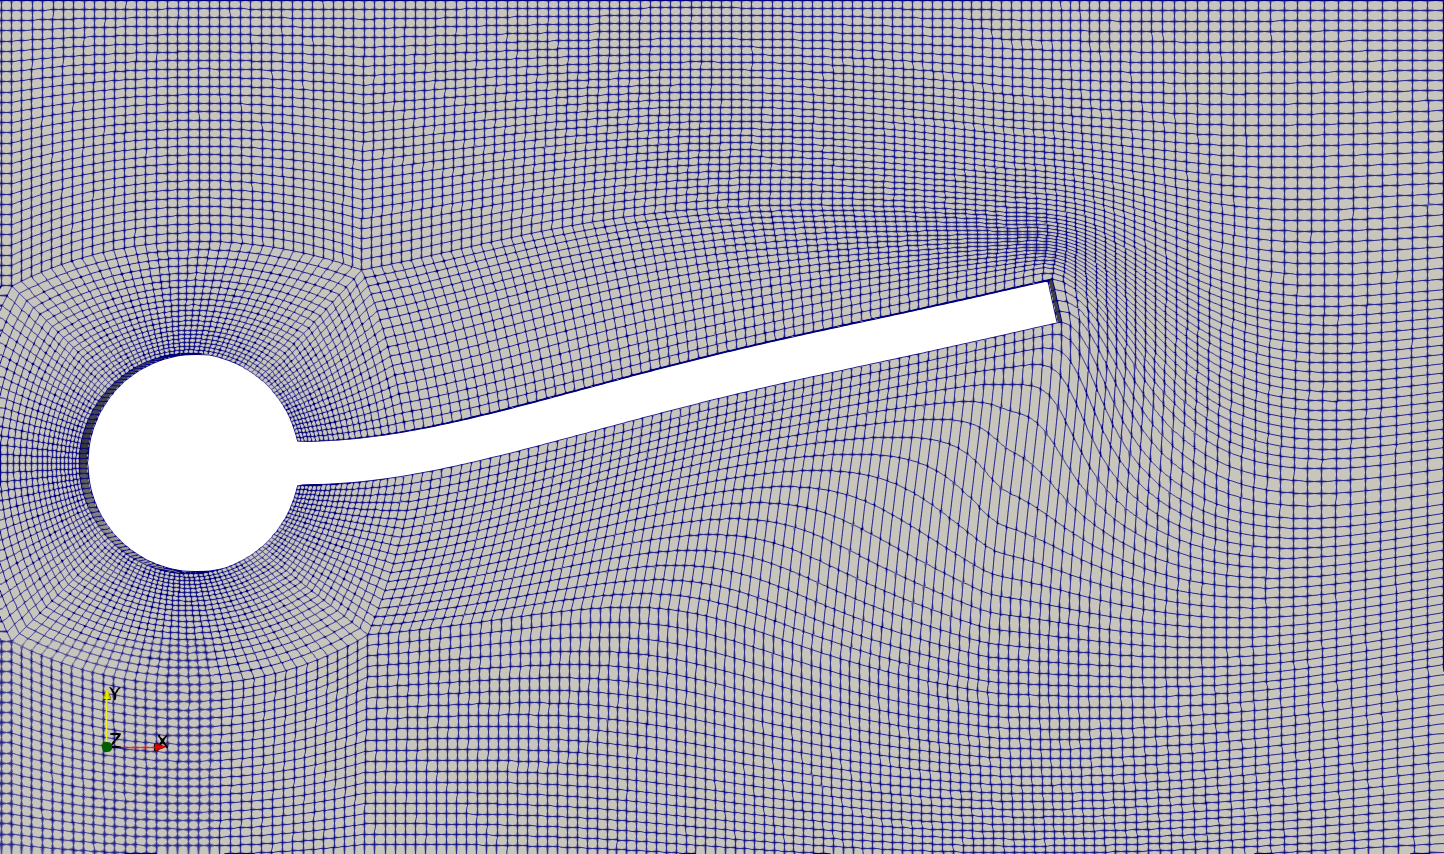
\includegraphics[width=3cm]{images/mesh/m01.png}}\hfil
\subfloat[$t=7.1s$]{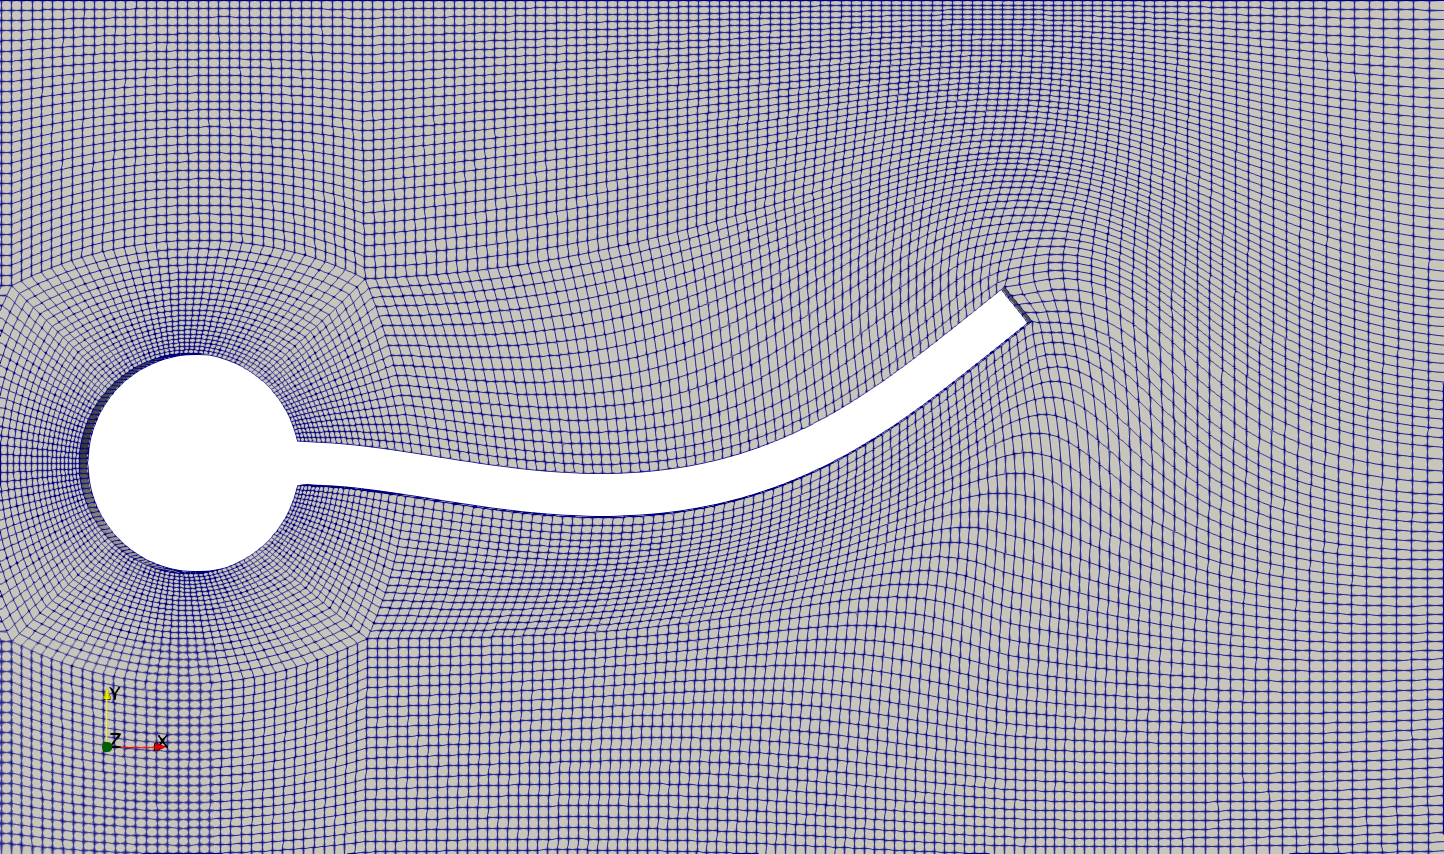
\includegraphics[width=3cm]{images/mesh/m02.png}}\hfil 
\subfloat[$t=7.2s$]{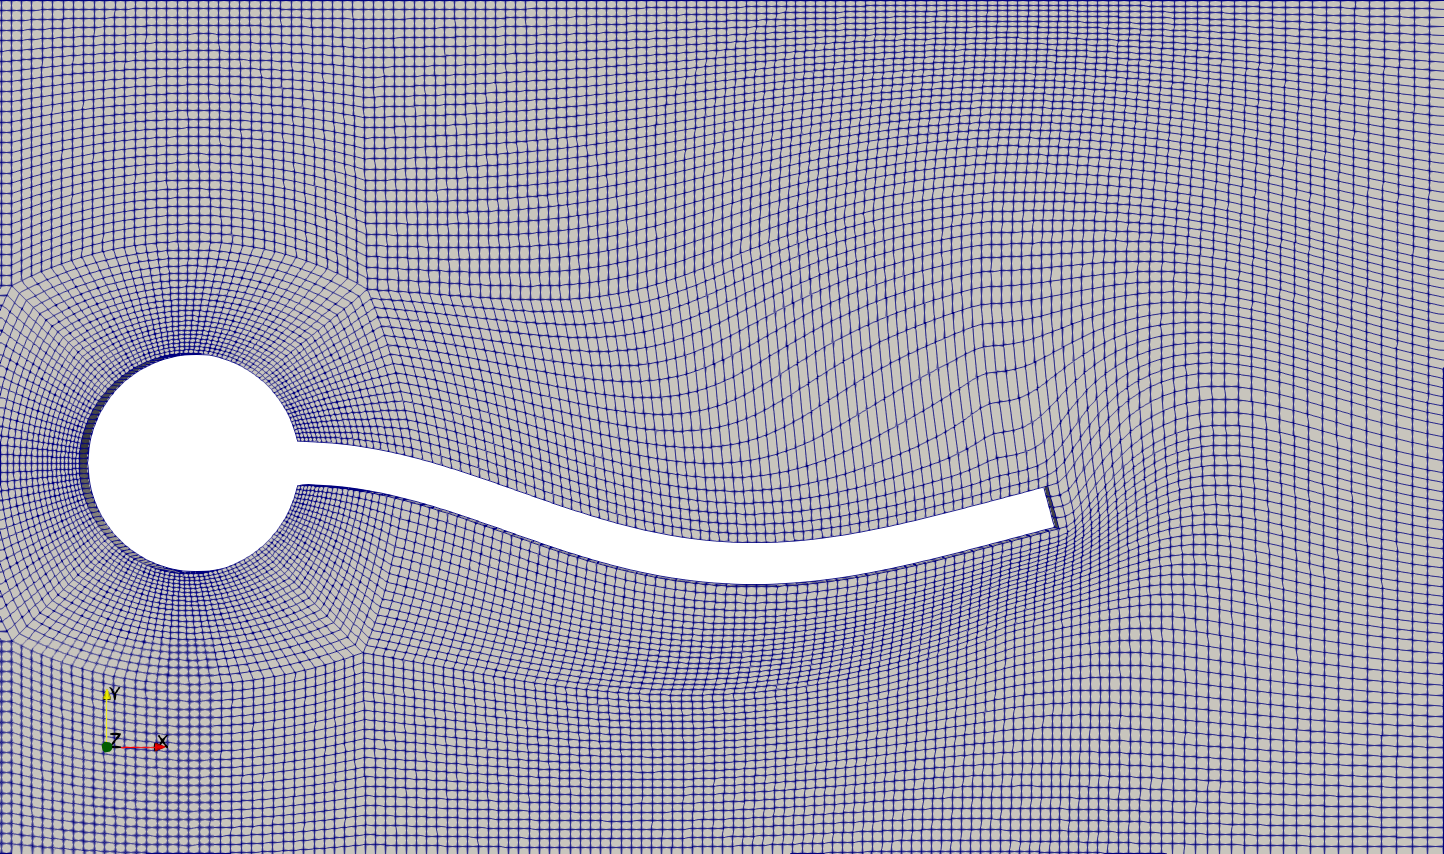
\includegraphics[width=3cm]{images/mesh/m03.png}} 

\subfloat[$t=7.3s$]{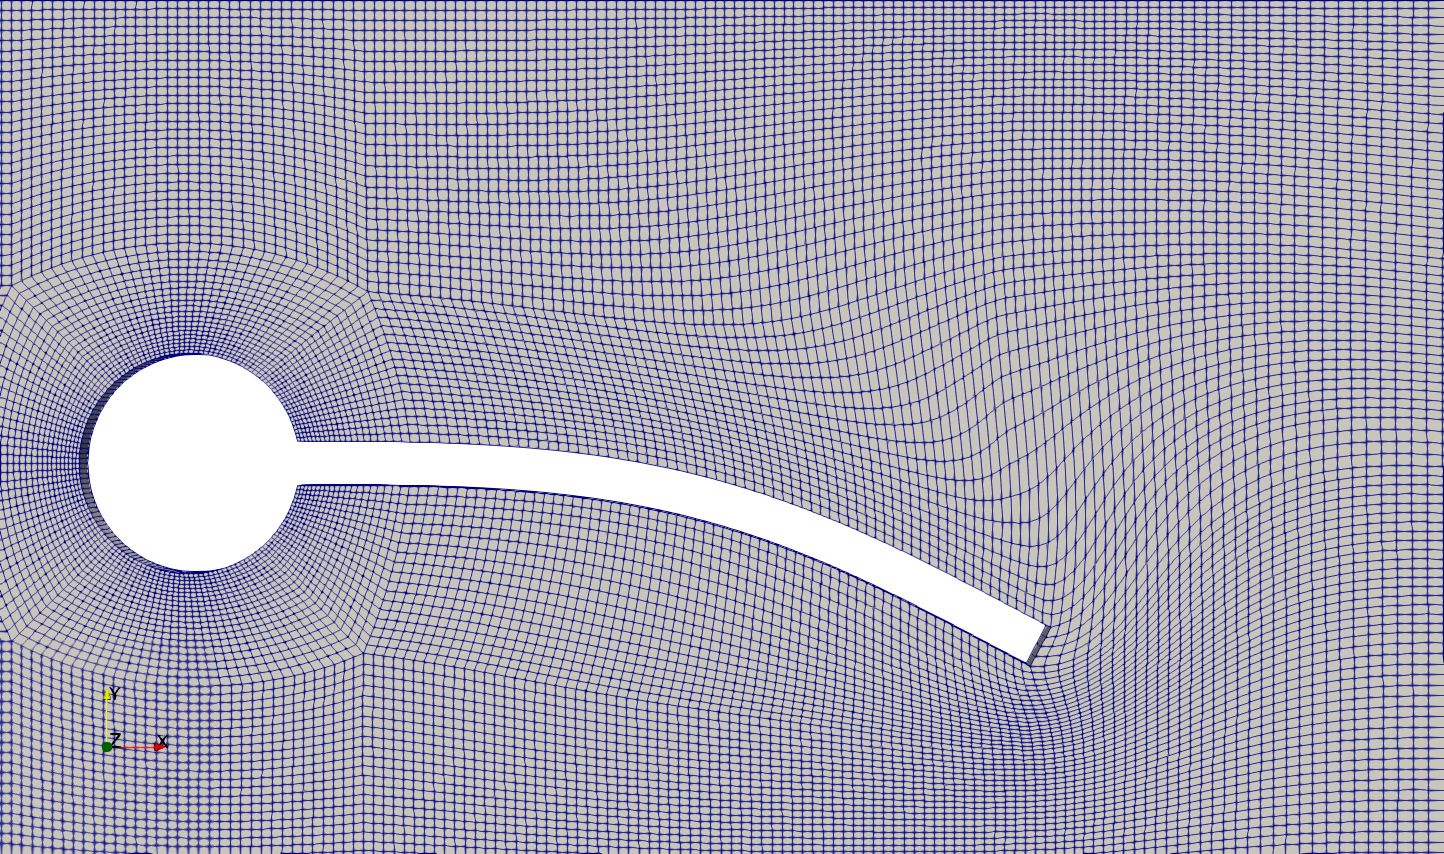
\includegraphics[width=3cm]{images/mesh/m04.png}}\hfil   
\subfloat[$t=7.4s$]{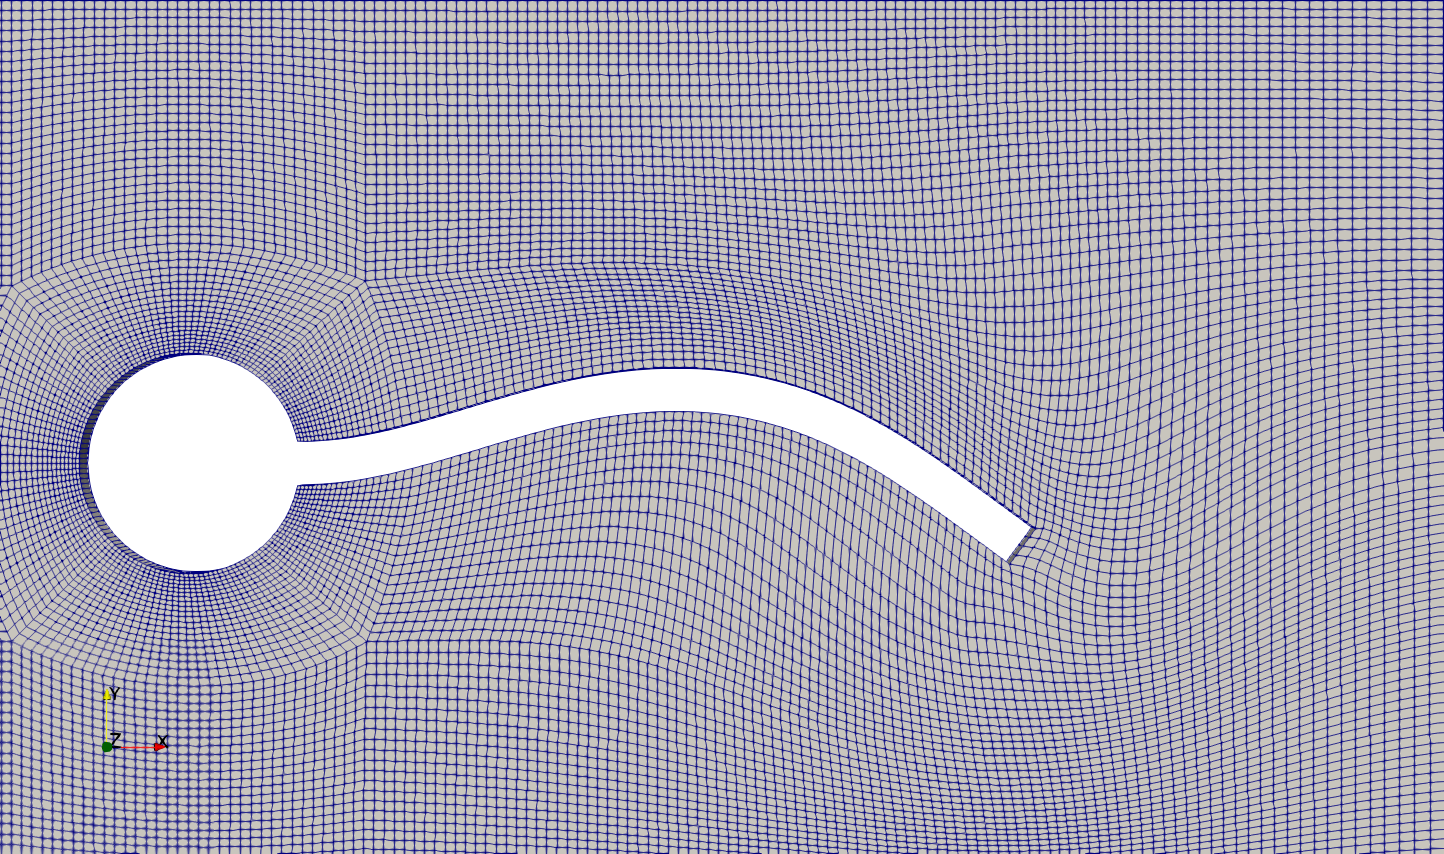
\includegraphics[width=3cm]{images/mesh/m05.png}}\hfil
\subfloat[$t=7.5s$]{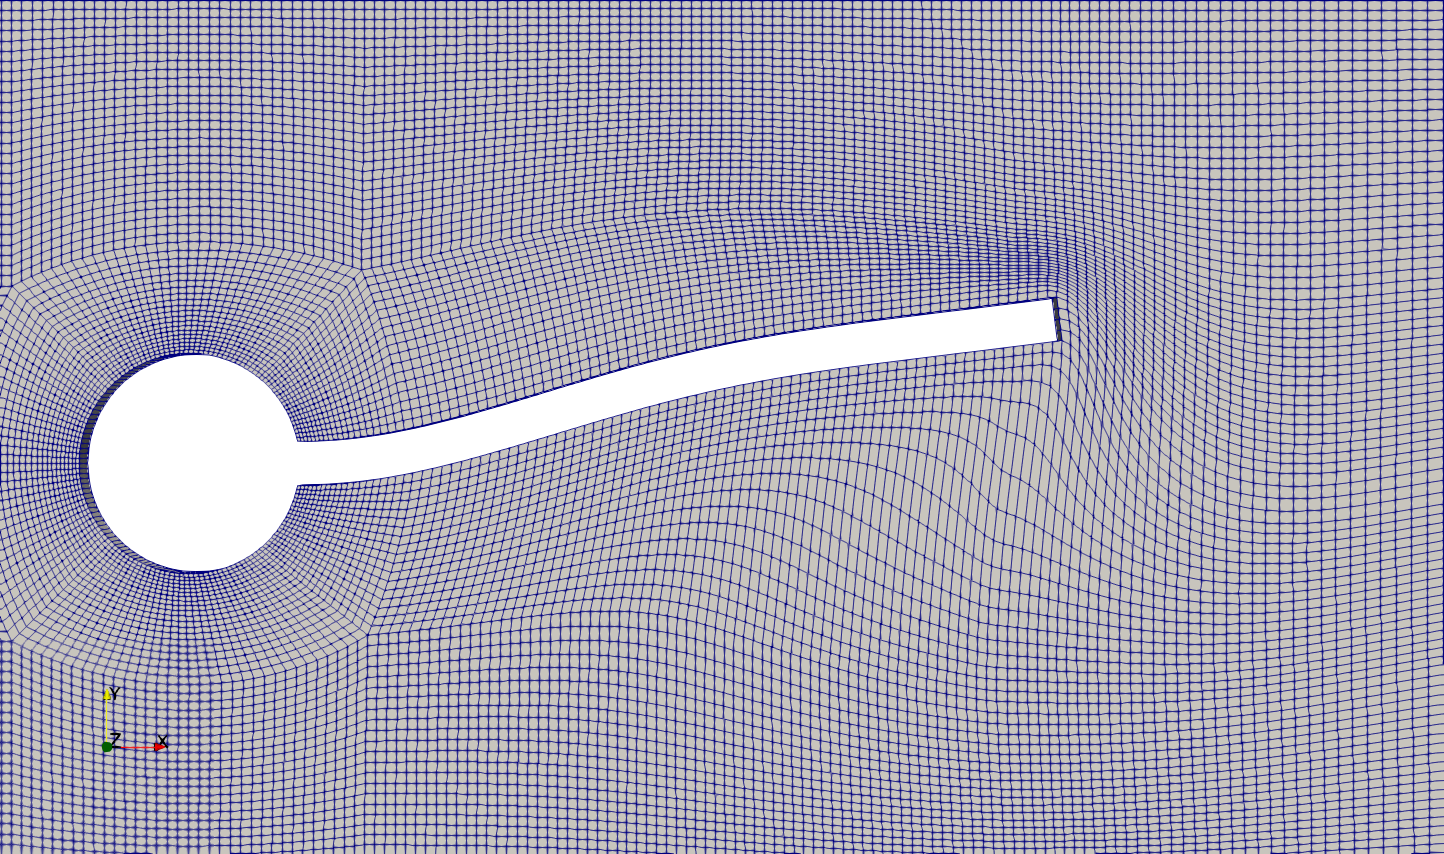
\includegraphics[width=3cm]{images/mesh/m06.png}}

\end{figure}
    
    
\end{frame}



\begin{frame}{Flapping wing: experimental setup}
\label{heathcote}
    \begin{columns}
    \column{0.5\textwidth}
        \begin{figure}
	    \centering
	        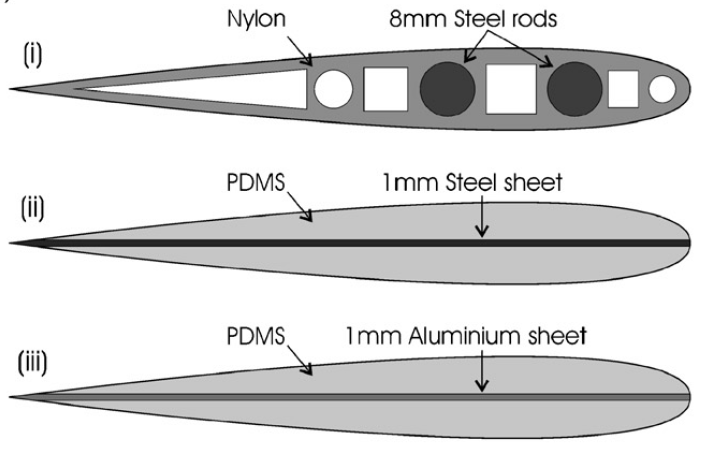
\includegraphics[width=0.8\textwidth]{images/heathcote/profiles0012}
	        \caption{wing section properties}
        \end{figure}

\footnotesize
\begin{itemize}
	\item $Re = \frac{\rho U_0 c}{\mu}$: $1\cdot10^4\div 3\cdot10^4$
	\item $k_G = \frac{\pi f c}{U_0}$: Garrick reduced fr. $0 \div 7$
	\item $S_r = \frac{2f a_{MID}}{U_0}$: at mid-span
\end{itemize}



    
    \column{0.5\textwidth}
        \begin{figure}
	    \centering
	        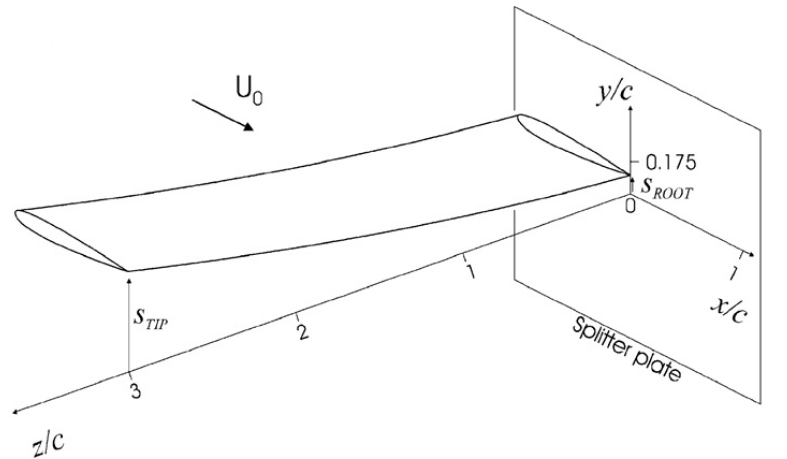
\includegraphics[width=0.87\textwidth]{images/heathcote/naca0012_exp}
	        \caption{experimental setup}
        \end{figure}

\footnotesize
\begin{itemize}
	\item $s = a_{ROOT} \sin(\omega t)$
	\item $C_T = \frac{T}{\frac{1}{2}\rho U_0^2c}$
	\item $\bar{C}_P = \frac{\bar{F_y v}}{\frac{1}{2}\rho U_0^3c}$
	\item $\frac{a_{TIP}}{a_{ROOT}}$ and  $\phi$
\end{itemize}


\end{columns}


\end{frame}


\begin{frame}{Flapping wing: simulation setup}
    \begin{columns}
    \column{0.5\textwidth}
        \begin{figure}
	    \centering
	        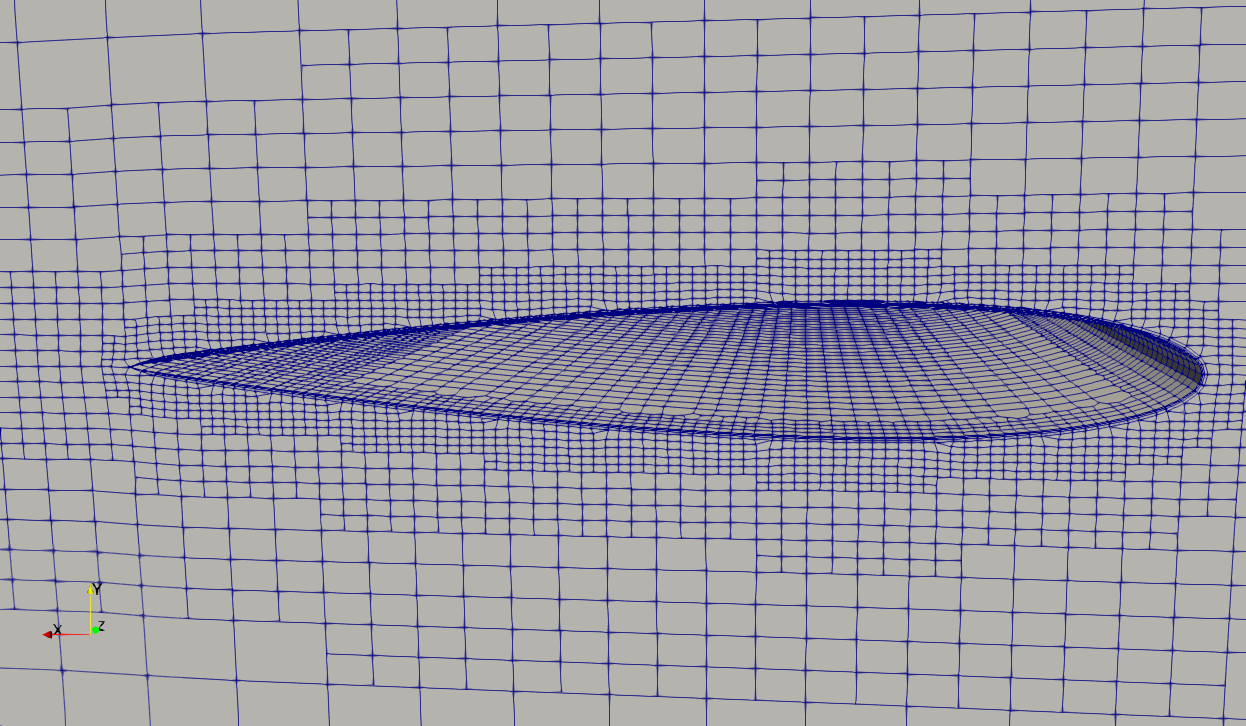
\includegraphics[width=0.8\textwidth]{images/heathcote/dom02.png}
	        \caption{fluid mesh}
        \end{figure}
        \vspace{0.25cm}
        \footnotesize
        \begin{itemize}
            \item $\approx 218k$ cells
            \item boundary conditions
            \item incompressible flow
        \end{itemize}

    \column{0.5\textwidth}
        \begin{figure}
	    \centering
	        \includegraphics[width=0.875\textwidth]{images/heathcote/interface01b.png}
	        \caption{interface mesh}
        \end{figure}
        \vspace{0.25cm}
        \footnotesize
        \begin{itemize}
            \item $\approx 1300$ interface cells
            \item 10 MBdyn \texttt{beam} elements
            \item stiffness given only by metal plate
            \item mass of plate and PDMS
        \end{itemize}
\end{columns}

\end{frame}


\begin{frame}{Flapping wing: preliminary results}

    \begin{columns}
    \column{0.5\textwidth}
        \vspace{-0.5cm}
        \begin{figure}
	    \centering
	        \includegraphics[width=0.98\textwidth, trim=0 60 0 60, clip]{images/heathcote/naca0012_disp.png}
	        \caption{tip displacement}
        \end{figure}
        \vspace{0.15cm}

    \column{0.5\textwidth}
        \footnotesize
        \begin{itemize}
            \item $\pm2.5$ mm @ 2.5Hz
            \item $Re=10000$, $k_G=0.785$, $S_r=0.015$
            \item $\frac{a_{TIP}}{a_{ROOT}} \approx 1.45$
            \item $\phi = 27^o$
            \item Model first eigenfrequency $6.8Hz$
            \item torsionally rigid $(< 0.1^o)$
        \end{itemize}

\end{columns}
\footnotesize
\textcolor{dorange}{\textbf{coupling}}:
\begin{itemize}
    \item staggered strong coupling
    \item acceleration: \textcolor{pblue}{IQN-ILS}
    \item mapping: \textcolor{teal}{RBF} or \textcolor{dblue}{nearest neighbor}
    \item avg. number of iterations: \textbf{18}
\end{itemize}

    
\end{frame}

\begin{frame}{Flapping wing: preliminary results}

    \begin{columns}

    \column{0.5\textwidth}
        \begin{figure}
        \vspace{-0.25cm}
	    \centering
	        \includegraphics[width=0.975\textwidth, trim=0 150 0 120, clip]{images/heathcote/forces_naca0012.png}
	        \caption{wing forces}
        \end{figure}

    \column{0.5\textwidth}
        \footnotesize
        \vspace{1.5cm}
        \begin{itemize}
            \item $\bar{C}_D\approx 0.02615$
            \item experimental $0.0245\div0.028$
            \item small Strouhal number to measure efficiency
        \end{itemize}
\end{columns}
    
\end{frame}

\begin{frame}{Flapping wing: images}
    \begin{figure}
    \centering
        \subfloat[velocity field $t=1.2s$]{\includegraphics[width=5cm]{images/heathcote/naca0012_U2.png}}\hfil
        %\subfloat[$t=7.1s$]{\includegraphics[width=3cm]{images/mesh/m02.png}}\hfil 
        \subfloat[pressure field $t=1.2s$]{\includegraphics[width=5cm]{images/heathcote/naca0012_p2.png}} 
        
        \subfloat[deformed shape (10x)]{\includegraphics[width=5cm, trim=0 100 0 0, clip]{images/heathcote/naca0012_dy.png}}\hfil   
        %\subfloat[$t=7.4s$]{\includegraphics[width=3cm]{images/mesh/m05.png}}\hfil
        \subfloat[$F_Y$]{\includegraphics[width=5cm, trim=0 100 0 0, clip]{images/heathcote/naca0012_Fy.png}}

\end{figure}
    
\hyperlink{fsi2}{\beamerreturnbutton{back}}
    
\end{frame}



\begin{frame}{FSI}
What is (not) FSI?
    \begin{columns}
        \column{0.5\textwidth}
        \begin{figure}
            \centering
            \includegraphics[width=0.95\textwidth]{images/valve.png}
            \caption{FEM with pressure load}
        \end{figure}
        \column{0.5\textwidth}
        \begin{figure}
            \centering
            \includegraphics[width=0.95\textwidth,trim=0 40 0 0,clip]{images/valve_cfd.png}
            \caption{CFD with moving domain}
        \end{figure}
    \end{columns}
    
    \pause
    
    \begin{enumerate}
        \item fluid represented as a pressure field
        
        \item solid considered rigid
    \end{enumerate}
    
    \vskip 5mm
    
   \textcolor{red}{Only one domain (solid/fluid) needs to be simulated}
    
    
\end{frame}

\begin{frame}{Turek-Hron FSI2 Benchmark: results}

\begin{columns}

\column{0.3\textwidth}
%\vspace{1cm}
and on\\ \textbf{overall lift and drag}:

\column{0.7\textwidth}


\vspace{-1cm}

\begin{figure}[htbp!]
    %\vspace{-1.8cm}
	\centering
	\includegraphics[width=0.9\textwidth, trim=20 40 20 20, clip]{images/FSI2/forces_fsi2_pres.png}
\end{figure}

\end{columns}

\footnotesize
\begin{center}
\begin{tabular}{ l | c c | c c  |  } 
	Study & drag \si{N.m^{-1}} & f \si{Hz} & lift \si{N.m^{-1}} & f \si{Hz}    \\ 
	\hline
	\hline
	Benchmark & $208.83\pm73.75$ & $3.8$ & $0.88\pm234.2$ & $2.0$     \\
	Turek et al. (2010) & $215.06\pm77.63$ & $3.86$ & $0.61\pm237.8$ & $1.93$\\   
	Gjertsen & $161.50\pm73.75$ & & $0.88\pm234.2$ & \\
	Degroote  & $217.52\pm84.65$ & $3.7$ & $-0.74\pm267.6$ & $1.9$ \\
	\hline
	Present study & $239.13\pm31.93$ & $3.87$ & $3.43\pm308.57$ & $1.93$ \\
\end{tabular}
    
\end{center}

\end{frame}





%{
%\usebackgroundtemplate{ \parbox[b][\paperheight][b]{\paperwidth}{\centering\includegraphics[width=\paperwidth]{Personal_BG/bp01mg.jpg}}} 
%\begin{frame}[plain,noframenumbering]
%    \titlepage
%\end{frame}
%}

%{
%\usebackgroundtemplate{ \parbox[b][\paperheight][b]{\paperwidth}{\centering\includegraphics[width=\paperwi%dth]{Personal_BG/bp01mc.jpg}}} 
%\begin{frame}[plain,noframenumbering]
%    \titlepage
%\end{frame}
%}



%{

%\usebackgroundtemplate{ \parbox[b][\paperheight][b]{\paperwidth}{\centering\includegraphics[width=\paperwidth]{Personal_BG/bp02mg.jpg}}} 
%\begin{frame}[plain,noframenumbering]
%    \titlepage
%\end{frame}
%}

%{
%\usebackgroundtemplate{ \parbox[b][\paperheight][b]{\paperwidth}{\centering\includegraphics[width=\pape%rwidth]{Personal_BG/cala02mg.jpg}}} 
%\begin{frame}[plain,noframenumbering]
%    \titlepage
%\end{frame}
%}

%{
%\usebackgroundtemplate{ \parbox[b][\paperheight][b]{\paperwidth}{\centering\includegraphics[width=\pape%rwidth]{Personal_BG/cala03mg.jpg}}} 
%\begin{frame}[plain,noframenumbering]
%    \titlepage
%\end{frame}
%}


%{
%\usebackgroundtemplate{ \parbox[b][\paperheight][b]{\paperwidth}{\centering\includegraphics[width=\paperwidth]{Personal_BG/ej01mg.jpg}}} 
%\begin{frame}[plain,noframenumbering]
%    \titlepage
%\end{frame}
%}

%{
%\usebackgroundtemplate{ \parbox[b][\paperheight][b]{\paperwidth}{\centering\includegraphics[width=\paperwidth]{Personal_BG/ej01mc.jpg}}} 
%\begin{frame}[plain,noframenumbering]
%    \titlepage
%\end{frame}
%}


%{
%\usebackgroundtemplate{ \parbox[b][\paperheight][b]{\paperwidth}{\centering\includegraphics[width=\paperwidth]{Personal_BG/ej02mg.jpg}}} 
%\begin{frame}[plain,noframenumbering]
%    \titlepage
%\end{frame}
%}

%{
%\usebackgroundtemplate{ \parbox[b][\paperheight][b]{\paperwidth}{\centering\includegraphics[width=\paperwidth]{Personal_BG/ej02mc.jpg}}} 
%\begin{frame}[plain,noframenumbering]
%    \titlepage
%\end{frame}
%}


%{
%\usebackgroundtemplate{ \parbox[b][\paperheight][b]{\paperwidth}{\centering\includegraphics[width=\paperwidth]{Personal_BG/ew01mg.jpg}}} 
%\begin{frame}[plain,noframenumbering]
%    \titlepage
%\end{frame}
%}

%{
%\usebackgroundtemplate{ \parbox[b][\paperheight][b]{\paperwidth}{\centering\includegraphics[width=\paper%width]{Personal_BG/ew02mg.jpg}}} 
%\begin{frame}[plain,noframenumbering]
%    \titlepage
%\end{frame}
%}

%{
%\usebackgroundtemplate{ \parbox[b][\paperheight][b]{\paperwidth}{\centering\includegraphics[width=\paper%width]{Personal_BG/ew03mg.jpg}}} 
%\begin{frame}[plain,noframenumbering]
%    \titlepage
%\end{frame}
%}

%{
%\usebackgroundtemplate{ \parbox[b][\paperheight][b]{\paperwidth}{\centering\includegraphics[width=\paperwidth]{Personal_BG/ew04mg.jpg}}} 
%\begin{frame}[plain,noframenumbering]
%    \titlepage
%\end{frame}
%}

%{
%\usebackgroundtemplate{ \parbox[b][\paperheight][b]{\paperwidth}{\centering\includegraphics[width=\paper%width]{Personal_BG/ew06mg.jpg}}} 
%\begin{frame}[plain,noframenumbering]
%    \titlepage
%\end{frame}
%}

%{
%\usebackgroundtemplate{ \parbox[b][\paperheight][b]{\paperwidth}{\centering\includegraphics[width=\paperwidth]{Personal_BG/ew07mc.jpg}}} 
%\begin{frame}[plain,noframenumbering]
%    \titlepage
%\end{frame}
%}


%{
%\usebackgroundtemplate{ \parbox[b][\paperheight][b]{\paperwidth}{\centering\includegraphics[width=\pape%rwidth]{Personal_BG/rotormg.jpg}}} 
%\begin{frame}[plain,noframenumbering]
%    \titlepage
%\end{frame}
%}


%{
%\usebackgroundtemplate{ \parbox[b][\paperheight][b]{\paperwidth}{\centering\includegraphics[width=\paperwidth]{Personal_BG/ry01mc.jpg}}} 
%\begin{frame}[plain,noframenumbering]
%    \titlepage
%\end{frame}
%}

%{
%\usebackgroundtemplate{ \parbox[b][\paperheight][b]{\paperwidth}{\centering\includegraphics[width=\paperwidth]{Personal_BG/ry02mg.jpg}}} 
%\begin{frame}[plain,noframenumbering]
%    \titlepage
%\end{frame}
%}

%{
%\usebackgroundtemplate{ \parbox[b][\paperheight][b]{\paperwidth}{\centering\includegraphics[width=\paperwidth]{Personal_BG/ry03mc.jpg}}} 
%\begin{frame}[plain,noframenumbering]
%    \titlepage
%\end{frame}
%}

%{
%\usebackgroundtemplate{ \parbox[b][\paperheight][b]{\paperwidth}{\centering\includegraphics[width=\paper%width]{Personal_BG/ry04mg.jpg}}} 
%\begin{frame}[plain,noframenumbering]
%    \titlepage
%\end{frame}
%}

%{
%\usebackgroundtemplate{ \parbox[b][\paperheight][b]{\paperwidth}{\centering\includegraphics[width=\pape%rwidth]{Personal_BG/ry05mg.jpg}}} 
%\begin{frame}[plain,noframenumbering]
%    \titlepage
%\end{frame}
%}

%{
%\usebackgroundtemplate{ \parbox[b][\paperheight][b]{\paperwidth}{\centering\includegraphics[width=\paper%width]{Personal_BG/ry06mg.jpg}}} 
%\begin{frame}[plain,noframenumbering]
%    \titlepage
%\end{frame}
%}


%{
%\usebackgroundtemplate{ \parbox[b][\paperheight][b]{\paperwidth}{\centering\includegraphics[width=\pape%rwidth]{Personal_BG/sky01mg.jpg}}} 
%\begin{frame}[plain,noframenumbering]
%    \titlepage
%\end{frame}
%}





\end{document}
